\chapter{Deep Learning}
This chapter summarizes the fundamentals of machine learning with a special focus on artificial neural networks. We will take a look at how these networks are built and how they can be trained. The term \textit{Deep Learning} actually refers to the structural size of these artificial networks in modern applications which are build from tens to hundreds of layers. \\
We will begin with some basic motivation and get familiar with terms and notation for machine learning in Section \ref{ssec:MLNutshell}. We then dive into the world of artificial neural networks and how they can be trained in Section \ref{sec:ANNs}, where we also talk about some of the most challenging problems for nowadays architectures and how they can be solved. Finally we will finish with some specialized network structures for specific applications in Section \ref{sec:SpecializedNetworks}.

\section{Machine Learning in a Nutshell} \label{ssec:MLNutshell}
In this Section we want to give an introduction into machine learning. We will begin with some motivation and talk about why machine learning matters in Section \ref{ssec:MLMotivation} and follow up with some basic terms and notation in Section \ref{ssec:MLNotation}.

\subsection{Motivation} \label{ssec:MLMotivation}
Before we dive into neural networks, let us briefly talk about what machine learning is and what makes it special. Machine learning is a field of study of computer science, which tries to give computers the ability to solve a task without a human writing an explicit algorithm for it. Usually machine learning works by providing \textit{training data} to a specialized learning algorithm which will then try to solve a task by optimizing a performance measure. For example think about a set of images, where on some of the images show apples and others show pears. When training, we split our \textit{dataset} into two - a larger one which will be our \textit{training dataset} and a smaller one which will be our \textit{test dataset}. Our algorithm will learn with the images from the training dataset only and for each sample gets the information what it can expect to see on the image. Its progress is then measured periodically in terms of \textit{accuracy} on the test dataset.

While we can expect a learned model to be fairly good, we can also expect to never reach a 100\% accuracy. Additionally machine learning is hard and time consuming so why do we not use traditional algorithms? Well first of all because there are many problems where traditional algorithms are either too complex or it does not even exist an algorithm to solve them. For example there is no known algorithm which precisely recognizes and classifies objects in an image. Machine learning can also be very dynamic. Imagine a spam detection engine. Traditional approaches worked with keyword filters which were simply lists of forbidden words (or sentences) created by humans. This approach required a lot of tedious work for a result which is not very robust, since someone who knows the filter list can try to simply use different words. In a setting where we use machine learning, we could let the computer create this list on its own. The only thing we would need to do is to tell it, which email contains spam and which does not. Machine learning can also go a step further and build a language model for us which allows to automatically detect synonyms - improving the robustness of the learned list. 

Machine learning is not only great at solving complex tasks, it can also help humans to learn. Machine learning is a great tool to find information in big piles of raw data. This area is called \textit{data mining} and can help to find unknown patterns to better understand problems.

\subsection{Terminology and Notation} \label{ssec:MLNotation}
In this Section we want to introduce some basic notation and terminology from the area of machine learning. We will further try to get a better view on what machine learning is from a mathematical point of view.

\paragraph{Types of Machine Learning.} Machine Learning is a very broad area and - depending on the task - very different techniques will be used.Therefore learning algorithms can usually be divided in (at least) three main categories:

\begin{enumerate}
  \item \textit{Supervised Learning.} Supervised learning algorithms aim at building a model from a training dataset where for each sample in the training dataset the desired output is given. Typical uses are classification or regression tasks.
  \item \textit{Unsupervised Learning.} Unsupervised learning algorithms try to find structure in a given dataset without the desired output. They are often used for clustering which is done by exploiting some similarity metric. Unsupervised methods can often be combined with supervised methods and then are called semi-supervised methods.
  \item \textit{Reinforcement Learning.} Reinforcement learning tries to train an agent to take actions in an environment to reach a certain goal. The agent is usually guided by some reward given to it which it will try to maximize. We will take a detailed look at reinforcement learning in Chapter \ref{chp: RLOverview}.
\end{enumerate}

\paragraph{Data Representation.} Data is not only a central element for every computer system, but also highly important for any machine learning algorithm. Without data, there is nothing we can learn from. Data can have arbitrary origin, but if the data comes from the real world it is usually collected by sensors. The data is often preprocessed and the algorithm gets the data in form of a vector representation $\mathbf{x} \in \mathbb{R}^n$ which we call the \textit{feature vector} $\mathbf{x}$ in the \textit{feature space} $\mathbb{R}^n$. These terms originate from the idea, that each dimension of the vector may contain a certain feature (e.g. weight and color of a fish), but we can also work on "raw" features like the values of pixels in an image. If we have a set of feature vectors (samples), we denote the whole set by $\mathbf{X}$. Data is crucially important for the performance of the model. The best algorithm will not be able to create a good model from a bad dataset. In particular datasets may be too small or unrepresentative to model a real distribution, the dataset might be be biased towards or against a certain group, or the samples of the dataset may not be independent which makes it hard to learn from them. Gathering good training data is therefore a central problem of machine learning.

\paragraph{Machine Learning Models.}
To solve a given task, machine learning algorithms build a model which is trained using the training data. We call a model which is done with its training process an \textit{inference} model, which is then used at \textit{test time} to solve the problem it has been trained for. There are currently a number of different models available, most prominent the artificial neural networks which we will discuss in the remainder of this chapter, but there are also other kinds of models like \textit{decision trees} or \textit{support vector machines}. All models are in some way parameterizable and we will denote their parameters with $\theta$. Depending on the task, models have a specific output, which is usually also in vector form and denoted by $\mathbf{y}$. For example if we look at classification tasks, the output vector usually contains probabilities for each class $i$. The model can then be seen as a function which outputs a probability $p(s = i| \mathbf{x})$ for every class given the feature vector $\mathbf{x}$. Using \textit{Bayesian Decision Theory}, simple models can be created by counting occurrences in the training dataset to estimate the likelihood $p(\mathbf{x}|s=i)$ and the prior $P(s=i)$. The class probability is then given by the bayes formula 

\[P(s=i|\mathbf{x}) = \frac{p(\mathbf{x}|s=i)P(s=i)}{p(\mathbf{x})}\]

The \textit{evidence} $p(\mathbf{x})$ is only a scaling factor which can be ignored when we are only interested in the class with the maximum likelihood for a given feature vector. Even though bayesian models are optimal, in very high dimensional and complex feature spaces it is not possible to model the likelihood and prior exactly, which is why most modern machine learning techniques estimate them. 

Of course there are many more applications for machine learning than classification, so the output of a model does not need to be a probability distribution over classes. Depending on the task the output might just be a single number, an image, a time series or an audio signal. There are no limitations.

\section{Artificial Neural Networks} \label{sec:ANNs}
In this Section we want to talk about \textit{Artificial Neural Networks} (ANNs) which is one of the most prominent model family for modern machine learning. We begin by giving a brief overview over their historical development in Section \ref{ssec:ANNHistory} and continue with their modern architecture in Section \ref{ssec:MLPs}. We will then look at how we can train neural networks with the famous backpropagation algorithm in Section \ref{sec:Backpropagation} and discuss an important component of ANNs - the activation functions - in Section \ref{ssec:ActivationFunctions}. Finally we will look at some of the biggest challenges regarding the training of neural networks in Section \ref{sec:NNChallenges}.

\subsection{History} \label{ssec:ANNHistory}
Technical advances were often inspired by carful observation of the nature around us. In most animals we can find neural cell structures which are connected in a specialized way to control muscles and process information from sensory cells. Neurons are also the building block for our own brain. Naturally the idea of recreating neurons to produce intelligent machines was interesting and explored since the early days of computer science. 

\begin{figure}[ht]
    
  \begin{center}
      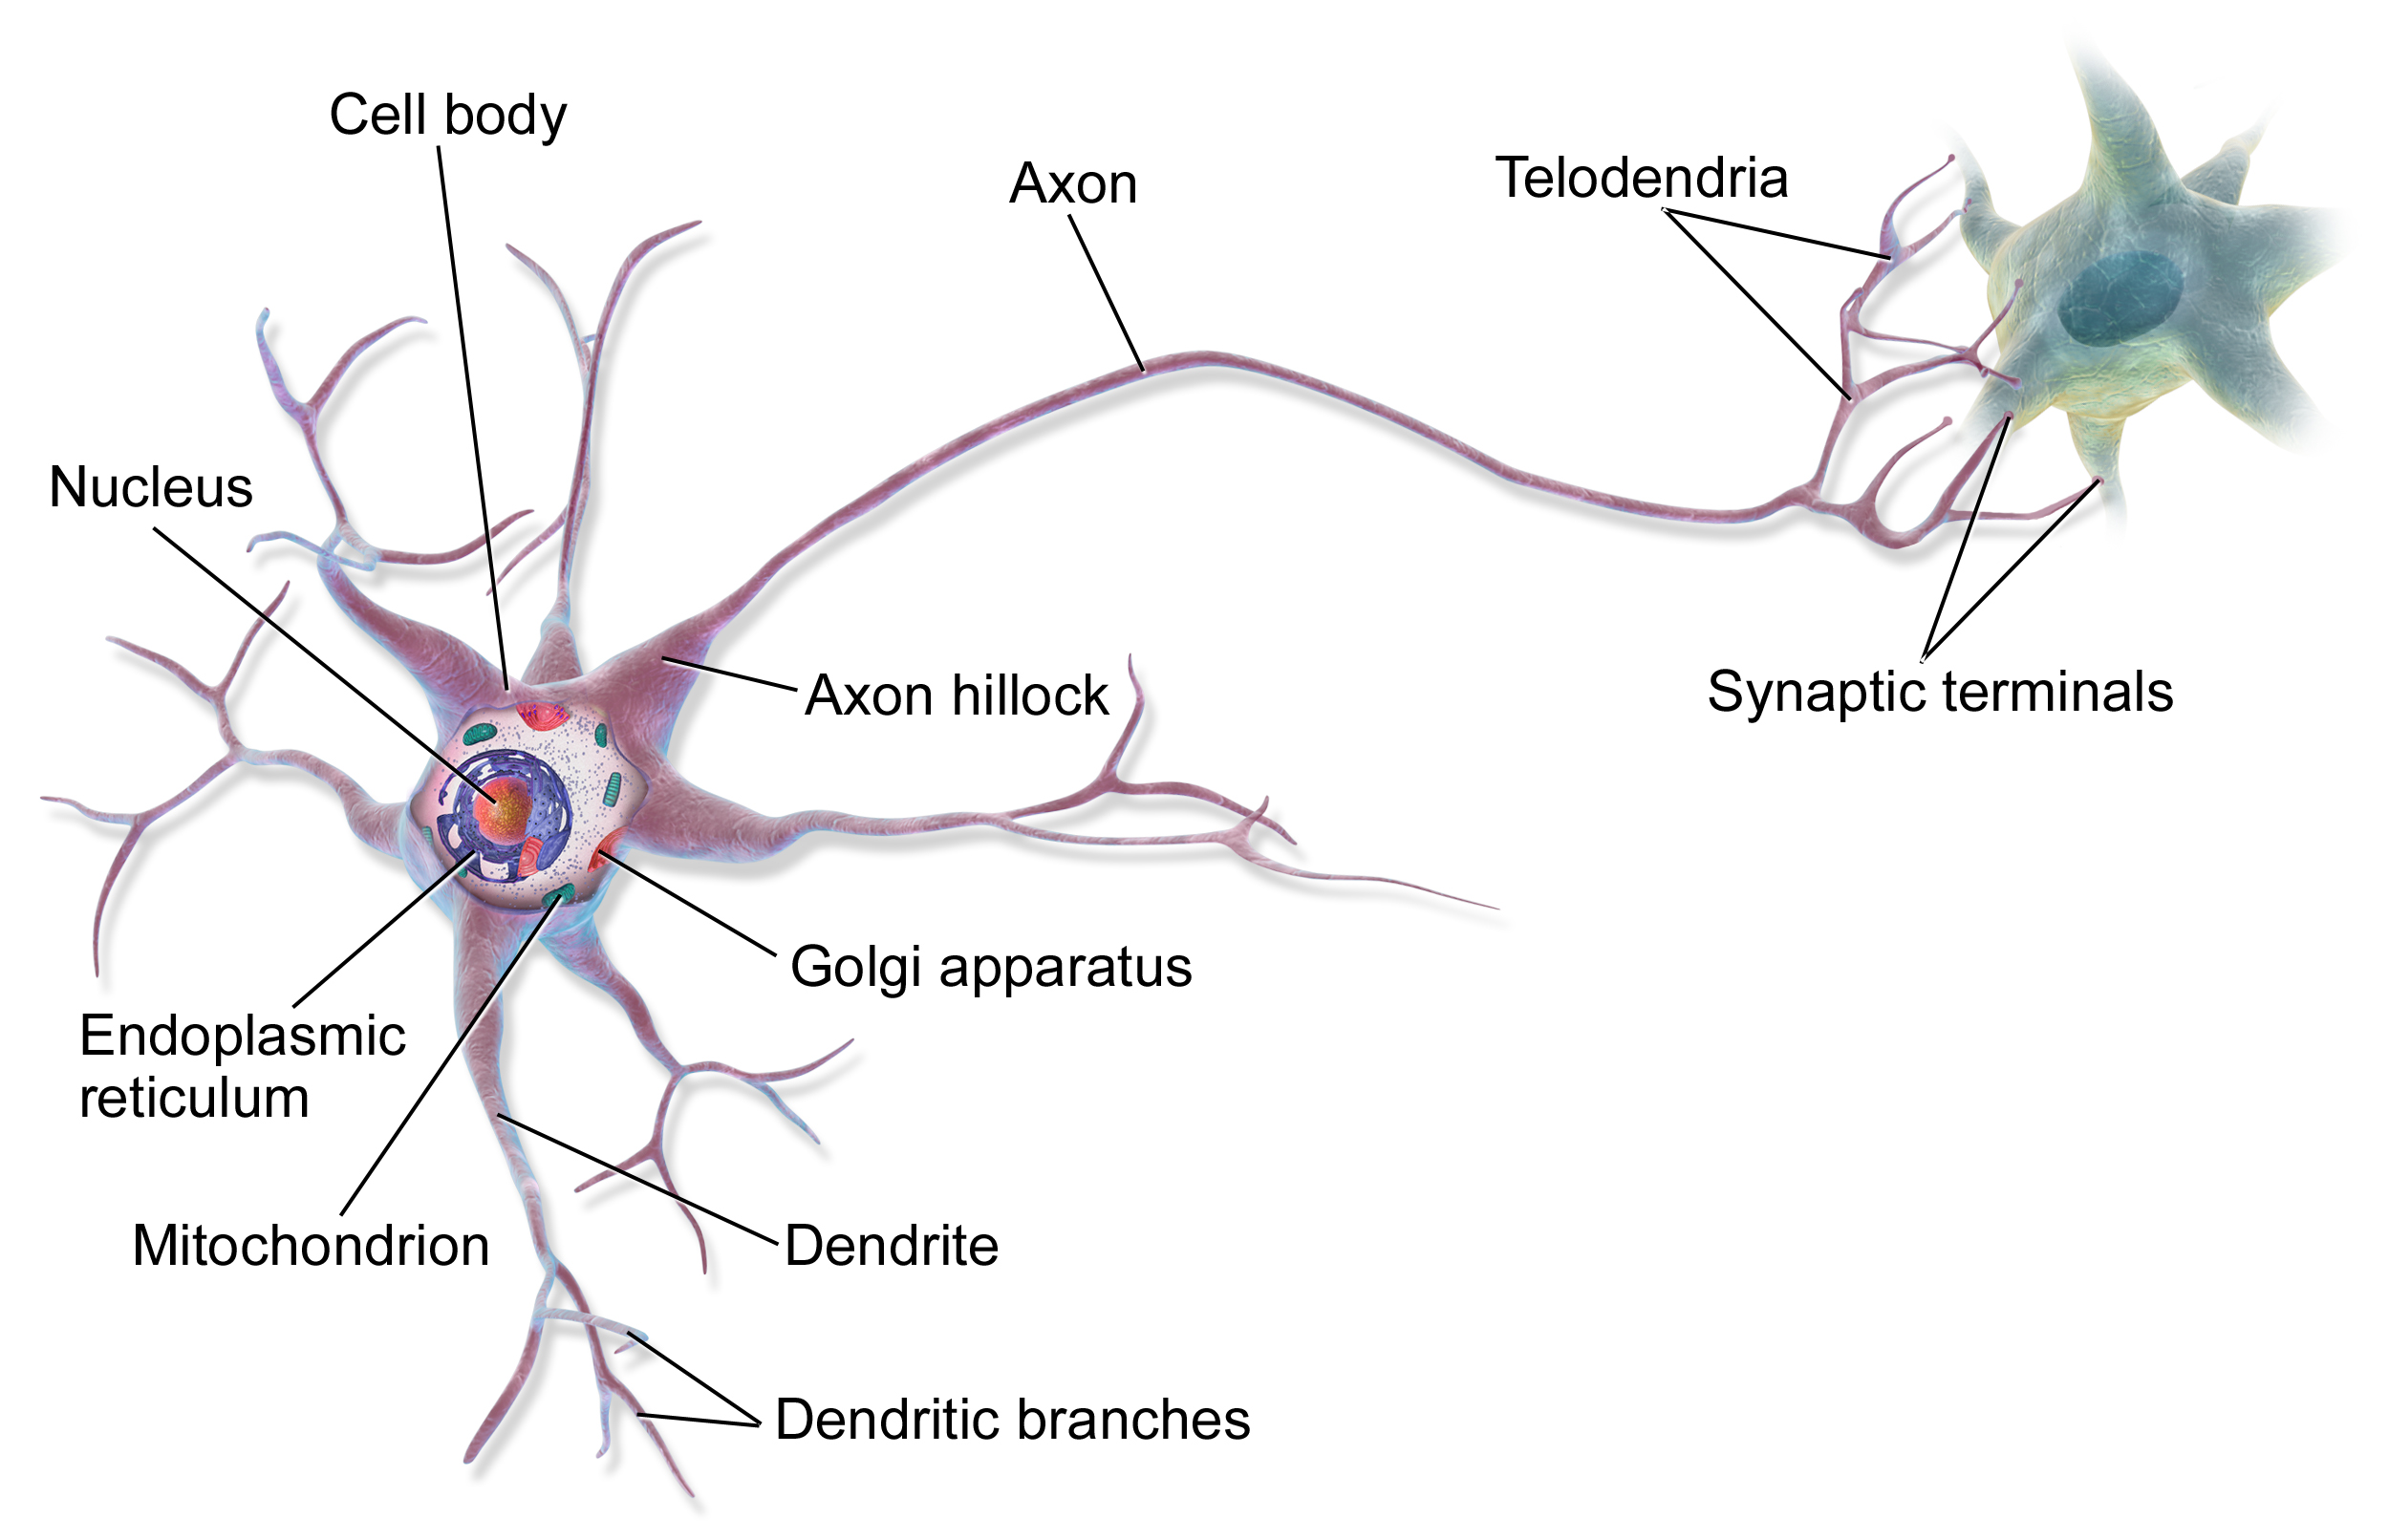
\includegraphics[clip, width=0.75\columnwidth]{figures/deeplearning/neuron.png}
  \end{center}
  
  %\vspace*{-6pt}
  \caption[Biological Neuron]{Biological Neuron\footnotemark}
  \label{fig:biological_neuron}
  %\vspace*{-12pt}
\end{figure}

\footnotetext{Image created by Bruce Blaus, released under Creative Commons under \url{https://commons.wikimedia.org/wiki/File:Blausen_0657_MultipolarNeuron.png}}

Before we look at the first artificial neuron, let us first take a look at its biological counterpart for which we included a sketch in Figure \ref{fig:biological_neuron}. Since the neuron is a specialized cell, it contains a cell body with a nucleus. Around its core, the neuron branches out into \textit{dendrites}. These dendrites can be seen as the inputs of the neuron. The output of the neuron is a single, long dendrite, called the \textit{axon}. The axon can have extremely different length, ranging from less than a millimeter up to meters. At its end, the axon branches out into \textit{telondendrias}, which end in \textit{synapic terminals} (also called \textit{synapses}). The synapses themselves are connected to the dendrites of other neurons or muscles. If the neuron receives a signal through its dendrites and the signal strength rises up to a certain level, the neuron answers by sending short electrical impulses called \textit{action potentials} (APs) down its axon. These APs result in neurotransmitters being released in the synapses - transmitting the signal to the next cell. Neurotransmitters are chemical substances which means, the electrical (digital) signal gets converted into an analog signal at the synapses. This signal at the synapses can lead to a further transmission of signals or inhibit the next neuron from firing. 

While a single biological neuron is fairly simple, neurons form extremely complicated structures. The human brain consists of around 86 billion neurons which work as a unit and form a lot of specialized substructures to control our body, process images from our eyes, or acoustic signals from our ears. Even more impressive is the fact, that these structures are not static and most of these capabilities can be learned and thus are flexible. Even though we do not understand all these processes in biological neurons in detail, we can try to use artificial version of these building blocks and experiment with them.

\begin{figure}[ht]
  \begin{center}
  \resizebox{0.95\columnwidth}{!}{%
  \begin{tabular}{cccc}
  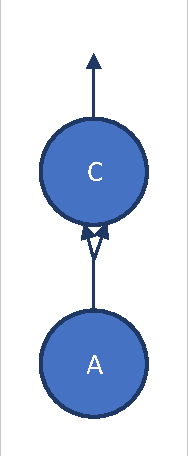
\includegraphics[clip, trim=10px 10px 10px 10px, height=5cm, page=1]{figures/deeplearning/ArtificialNeuron.pdf}  &
  \includegraphics[clip, trim=10px 10px 10px 10px, height=5cm, page=2]{figures/deeplearning/ArtificialNeuron.pdf} & 
  \includegraphics[clip, trim=10px 10px 10px 10px, height=5cm, page=3]{figures/deeplearning/ArtificialNeuron.pdf} &
  \includegraphics[clip, trim=10px 10px 10px 10px, height=5cm, page=4]{figures/deeplearning/ArtificialNeuron.pdf}\\
  {$C = A$} &
  {$C = A \wedge B$} &
  {$C = A \vee B$} &
  {$C = A \wedge \neg B$}\\
  
  \end{tabular}
  }%
  \end{center}
  %\vspace*{-12pt}
  \caption[Artificial Neurons for Logical Expressions]{Artificial neurons for logical expressions. The neurons (circles) A, B compute the output C via connections (arrows).}
  \label{fig:ArtificialNeuron}
  %\vspace*{-12pt}
\end{figure}

The first version of this artificial neuron was proposed early in 1943 by Warren McCulloch and Walter Pitts \cite{mcculloch1943logical}. They showed how logical expressions can be build with a network of binary neurons. Logical neurons activate their output if at least two of their inputs are active. Figure \ref{fig:ArtificialNeuron} shows an example for the basic logical operations \textit{and}, \textit{or} and \textit{not}. It is clear, that we can express arbitrary logical formulas in conjunctive or disjunctive normal form using these neurons. However neurons which only support binary values are not able to compute functions which is a major shortcoming. McCulloch and Pitts therefore also proposed a second version: The \textit{Threshold Logic Unit} (TLU). TLUs are able to perform continuous linear function computations. They achieve this by first computing a weighted sum of the inputs $z = w_1x_1 + w_2, x_2 + \dots + w_n, x_n = \mathbf{x}^T\mathbf{w}$ and then applying a step function. This step function sets the output to $+1$ if $z\geq0$ and otherwise to $0$. We included a graphical version which shows a single TLU in Figure \ref{fig:TLU}. The behavior of the step function matches the behavior of biological neurons, which either fire their signal at full signal strength or do not fire at all. A single TLU is able to perform binary classification tasks (output is either $1$ or $0$ depending on the class). Training the TLU then means to find the right weights for each input. The question is how to find these weights?

\begin{figure}[ht]
  
  \begin{center}
      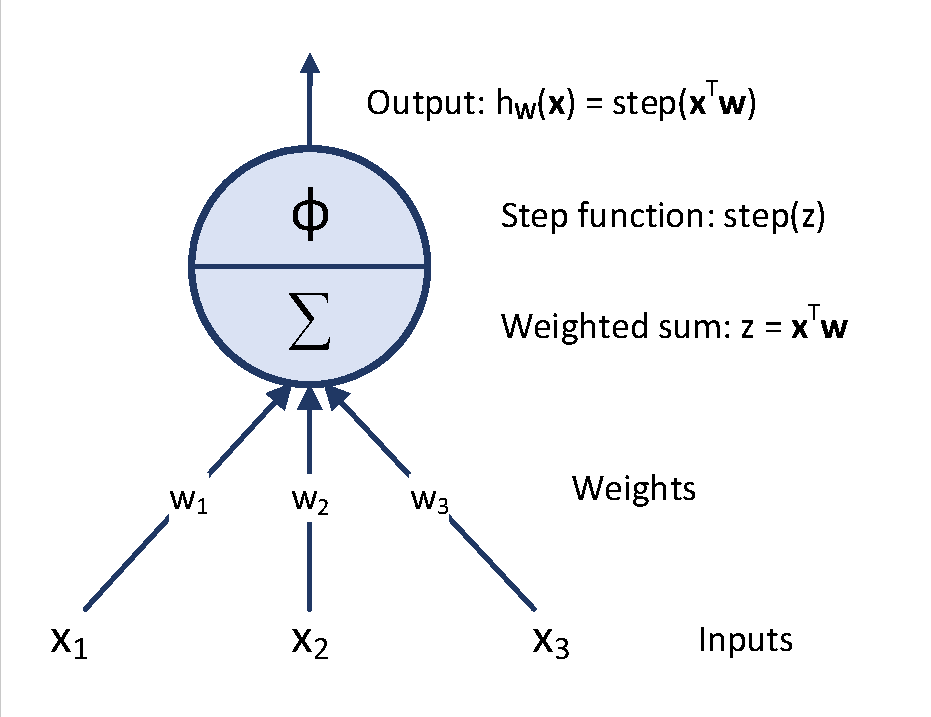
\includegraphics[trim=10px 10px 10px 10px, clip, width=0.5\columnwidth]{figures/deeplearning/TLU.pdf}
  \end{center}
  
  %\vspace*{-6pt}
  \caption[Threshold Logic Unit]{A \textit{threshold logic unit} is an artificial neuron which computes its output by a weighted sum of its inputs and a special step function.}
  \label{fig:TLU}
  %\vspace*{-12pt}
\end{figure}

 In 1957 Frank Rosenblatt invented the \textit{Perceptron} as an extension of the TLU. A perceptron is a combination of multiple TLUs to a layer of neurons, which all are connected to the inputs. We included an example in Figure \ref{fig:Perceptron}. Usually a bias neuron is added to the inputs to give the network more flexibility. The neurons in the first layer build the \textit{input layer} and just pass the input signal to the neurons in the \textit{output layer}. Both layers are \textit{fully connected} meaning every neuron in the input layer is connected to every neuron in the output layer. The output of the output layers TLUs can be computed at once by 

 \[h_{\mathbf{W}, \mathbf{b}}(\mathbf{X}) = \phi(\mathbf{XW} + \mathbf{b})\]

where $\mathbf{X}$ represents the input, $\mathbf{W}$ is a concatenation of all the weights of the TLUs (except for the bias neurons) and $\mathbf{b}$ represents the bias. For now the function $\phi$ is the step function. 

\begin{figure}[ht]
  
  \begin{center}
      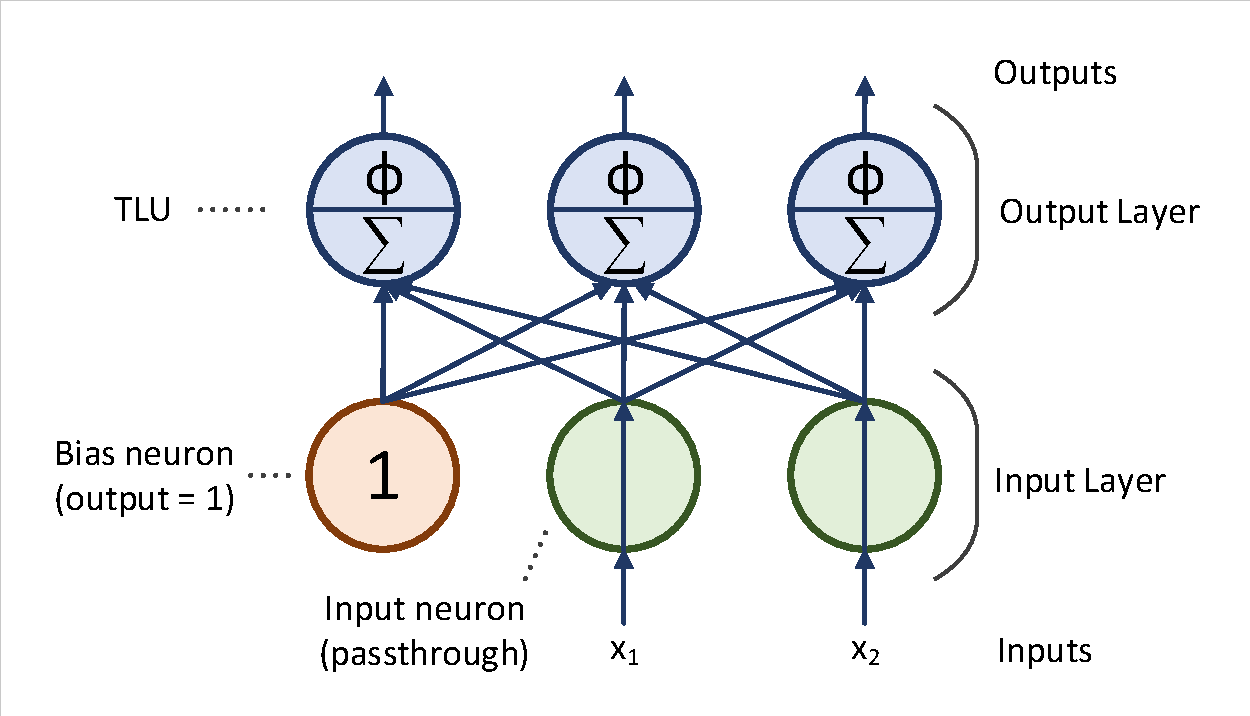
\includegraphics[trim=10px 10px 10px 10px, clip, width=0.7\columnwidth]{figures/deeplearning/Perceptron.pdf}
  \end{center}
  
  %\vspace*{-6pt}
  \caption[Perceptron Example]{Example for a \textit{perceptron} with 2 neurons and a bias in the input layer and 3 neurons in the output layer.}
  \label{fig:Perceptron}
  %\vspace*{-12pt}
\end{figure}

Rosenblatt also proposed a simple algorithm which is able to compute the weights for all TLUs for a given classification problem based on the error the network made. This algorithm is based on the perceptron learning rule 

\[w_{i, j}^{new} = w_{i, j} + \eta(y_j - \hat{y}_j) x_i\]

After the network classified the examples $x_i$, it updates the weights depending on the outcome - $y_j$ is the current output of the $j$th neuron and $\hat{y}_j$ the target value. The weights $w_{i, j}$ describe the weights between the $i$th input neuron and the $j$th output neuron. The parameter $\eta$ is the \textit{learning rate} for the network. The perceptron originally was build as a pure hardware implementation. The machine was connected to a camera and was one of the first machines which was able to learn weights for image recognition. \\
In 1969 it was proven by Marvin Minsky and Seymour Papert, that perceptrons are only able to compute linear functions and cannot compute a logical XOR from their inputs. Therefore perceptrons can only be used for simple linear classification tasks. However if the data is linearly separable, perceptrons are proven to converge.

\subsection{Multi-Layer Perceptrons} \label{ssec:MLPs}
So how do we actually learn nonlinear separation with TLUs if perceptrons are unable to do so? A simple but powerful extension to the original idea was to just stack multiple perceptrons on top of each other as shown in Figure \ref{fig:MLP}. 

\begin{figure}[ht]
  
  \begin{center}
      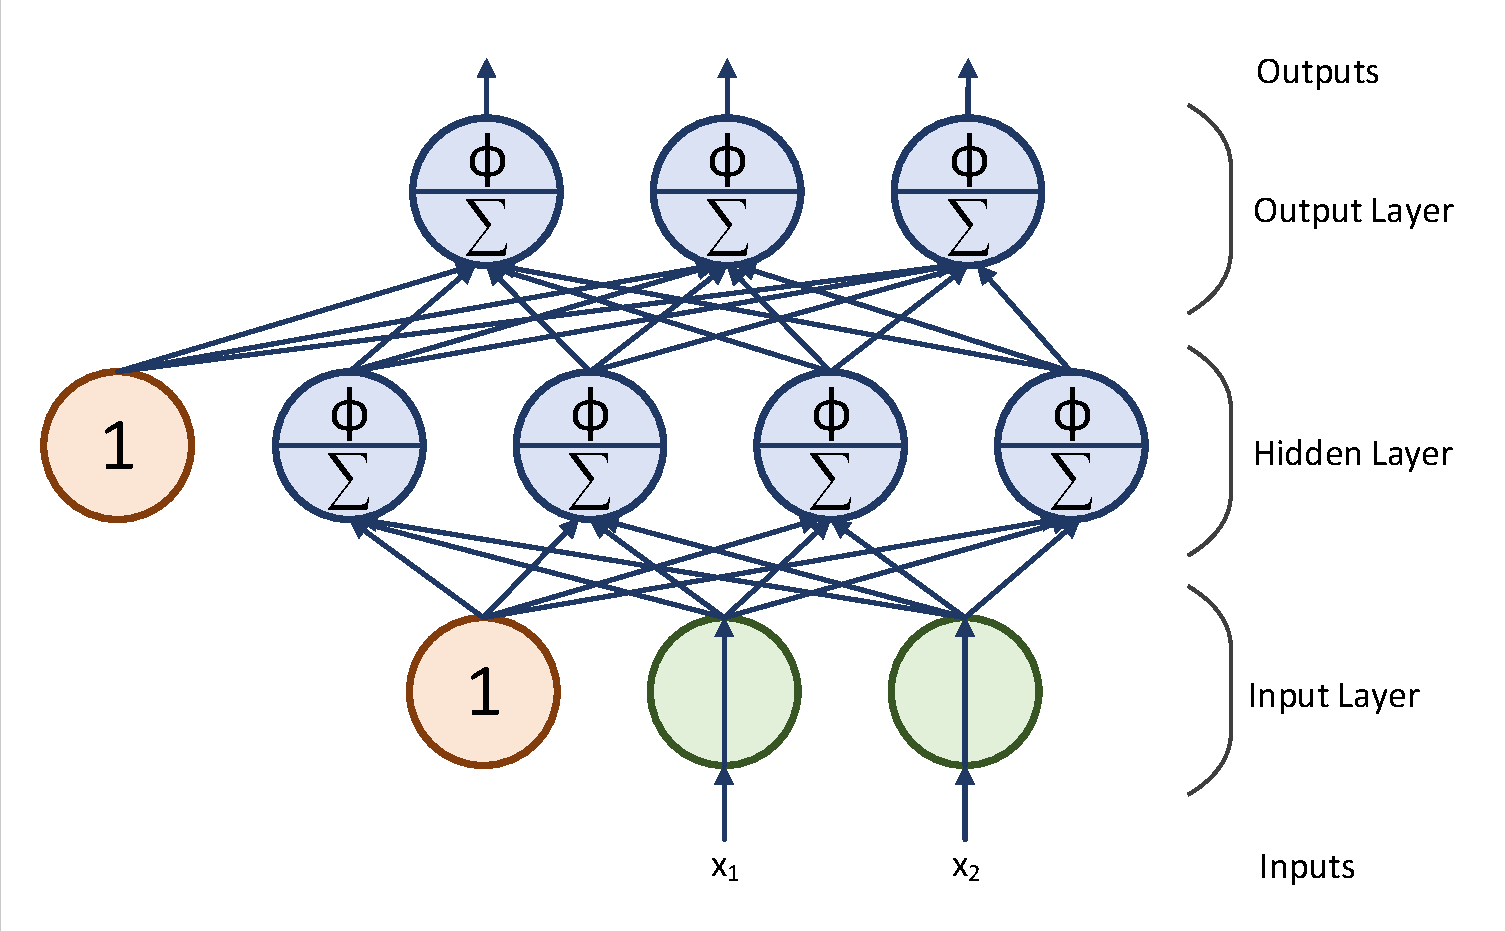
\includegraphics[trim=10px 10px 10px 10px, clip, width=0.8\columnwidth]{figures/deeplearning/MLP.pdf}
  \end{center}
  
  %\vspace*{-6pt}
  \caption[Multi-Layer Perceptron Example]{Example for a \textit{multi-layer perceptron} network with 2 neurons and a bias in the input layer and 4 neurons and a bias in the hidden layer and 3 neurons the output layer. The number of hidden layers and neurons per layer in a network can be arbitrary large.}
  \label{fig:MLP}
  %\vspace*{-12pt}
\end{figure}

This extended network actually allows to compute the XOR operation. Layers between the input and the output layer are called \textit{hidden layers} since they have no connection to the outside world. Computations are done layerwise similar to perceptrons by computing $h_{\mathbf{W}, \mathbf{b}}(\mathbf{X}) = \phi(\mathbf{XW} + \mathbf{b})$ for each layer, where $\mathbf{X}$ is the output of the previous layer. Each layer may have an individual number of neurons. The name deep learning rises from the idea of stacking more and more layers on top of each other to build \textit{deep neural networks} (DNNs). Because the input "flows" directly from the input to the output through each layer, these networks are also called \textit{Feedforward Neural Network} (FNN). The idea of stacking multiple perceptrons on top of each other was known for quite some time, but the problem was that it has been unclear how these networks could be trained. The simple perceptron algorithm does not work anymore, cause we now need to compute the error with respect to every layer. Additionally even though stacked perceptrons are able to compute XOR operations they are still limited to learning linear functions, since they are only a combination of other linear functions.

\subsection{Gradient Descent and Backpropagation} \label{sec:Backpropagation}
It took a few years, until in 1985 Rumelhart et al. were able to develop an algorithm to train multilayer networks while simultaneously introducing nonlinearity \cite{rumelhart1985learning}. Their algorithm combines the idea of \textit{gradient descent} with a method called \textit{backpropagation} which allows to calculate gradients for the weights of each layer of the network.

\begin{figure}[ht]
  
  \begin{center}
      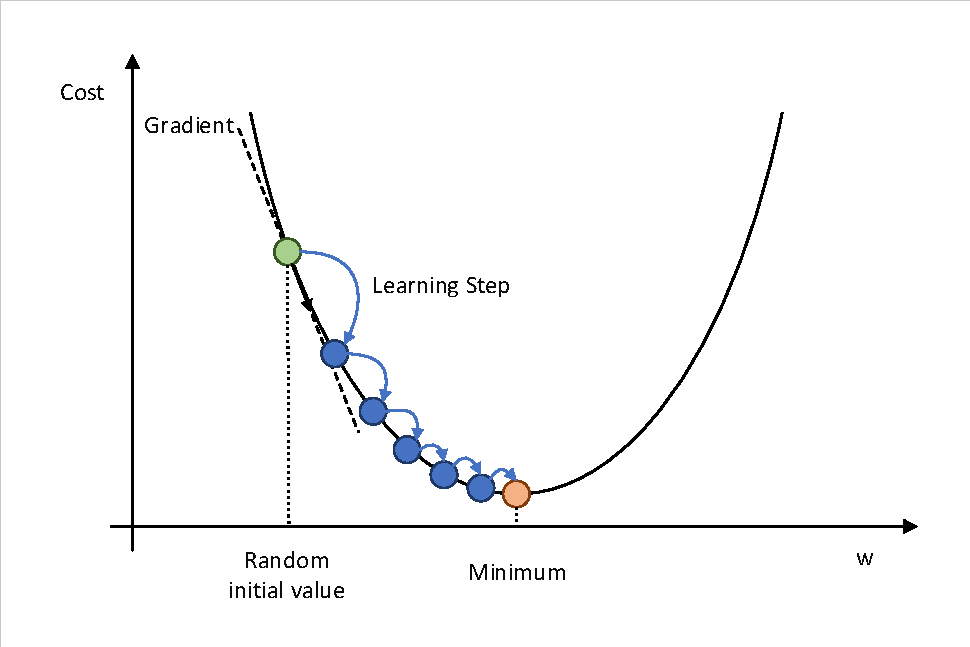
\includegraphics[trim=10px 10px 10px 10px, clip, width=0.75\columnwidth]{figures/deeplearning/GradientDescent.pdf}
  \end{center}
  
  %\vspace*{-6pt}
  \caption[Gradient Descent]{The idea of gradient descent.}
  \label{fig:GradientDescent}
  %\vspace*{-12pt}
\end{figure}

\paragraph{Gradient Descent.} Let us first look the gradient descent. Gradient descent is a method to calculate the minimum of a function. Given an arbitrary starting point on the function, gradient descent will iteratively find a series of new points leading towards a minimum (see Figure \ref{fig:GradientDescent}). Suppose we are at some point $x_k$ on our function $f$, we can then calculate the next step using the gradient $\nabla f$ of our function. We therefore can calculate 

\begin{align*}
  \delta_k &= -D_k \nabla f(x_k) \\
  \text{and } x_{k+1} &= x_k + \eta_k \delta_k
\end{align*}

as the next point closer to the minimum. The parameter $\eta$ is known as step size and in the context of deep learning is referred to as \textit{learning rate}. Usually at each step we are interested to calculate the steepest descent at the current point, since this will lead us quickly to our minimum, therefore we set $D_k = I$, with $I$ being the identity matrix. Note that there exist other approaches for second order optimization which use Hessians for $D_k$ instead.

The choice of an appropriate $\eta$ is crucial for gradient descent. Too large values will lead to points which oscillating around the minimum or even completely diverge from it, while too small values for $\eta$ might need many iterations to converge. Gradient descent also does not guarantee convergence to a global minimum and smaller learning rates increase the danger of getting stuck in a local minimum.

We now know what gradient descent does, but the question is which function can we minimize in the context of machine learning and how do we train a model by doing so? If we look at a neural network, it outputs a vector $\mathbf{z}$ at its output layer. This output is usually desired to give us some information (e.g. class probabilities in a classification task). When training we know the true output vector $\mathbf{y}$ the network should produce for some given input. Therefore we can calculate the error of the network in terms of a cost function over the dataset. Depending on the task there are several different cost functions which can be used. One of the most common ones is the \textit{mean squared error} (MSE):

\begin{equation*}
  MSE(\mathbf{x}, \theta) = \frac{1}{n} \sum^n_{i=1} (z_i - y_i)^2
\end{equation*}

Since the output vector $\mathbf{z}$ is dependent on the input vector $\mathbf{x}$ and the network weights $\theta$, but we only have control over $\theta$, we often write $MSE(\mathbf{x}, \theta)$ as $MSE(\theta)$ for short. When performing gradient descent we then calculate the gradient with respect to $\theta$. 

When implementing gradient descent for neural networks, we are sometimes interested in optimizing for multiple objectives at once. We therefore usually perform gradient decent with respect to a so-called loss function $\mathcal{L}(\theta)$ (which is equal to our cost function at the moment). We then denote the gradient of that function with respect to the network weights as $\nabla_\theta \mathcal{L}(\theta)$. A single gradient descent step for our network is then given by

\begin{equation*}
  \theta^{new} = \theta - \alpha \nabla_\theta \mathcal{L}(\theta)
\end{equation*}

Because the calculations for the gradient descent step are costly, it is usually considered sufficient to only calculate the gradient for a single sample from the dataset in each step (as opposed to calculating the gradient as a mean over the whole dataset). This procedure is called \textit{stochastic gradient descent} (SGD) and is a stochastic approximation of gradient descent. Training with SGD is less stable, but much faster. To stabilize training, SGD often uses \textit{minibatches} of data, where the gradient is calculated over a smaller batch of samples instead with a single sample.

\paragraph{Backpropagation.} Now that we know how we can calculate updates for the neural network, we need to know how it is possible to update the weights for each individual layer. This is where the \textit{backpropagation algorithm} comes in place. It mainly consists out of two phases: A forward pass, which allows us to determine the error (e.g. using MSE) and a backwards pass which determines which layer was involved to which extend with the error.

Let us look at the phases in more detail. The forward pass takes a sample (or a batch of samples) and propagates them through the network. For each layer, we collect the output activations and store them for later. After passing the input through the network and the calculation of the final output, we calculate our error like before. 

In second phase we begin at the output layer and propagate the error backwards layer by layer. This is done by calculating the weight change $\Delta w_{i, j}$ from neuron $i$ from the previous layer to neuron $j$ from the current layer by:

\begin{align*}
  \Delta w_{i, j} &= -\eta \delta_j o_i \\
  \text{with } \delta_j &= \begin{cases}
    \varphi'(v_i)(o_j - y_j) & \text{if $j$ is in the output layer}  \\
    \varphi'(v_i) \sum_k \delta_k w_{j,k} & \text{if $j$ is in a hidden layer}
  \end{cases}
\end{align*}

where the subscript always defines the number of the neuron in the layer. If the subscript is an $i$ we reference the previous layer (closer to the inputs) and $j$ references the current layer. We denote $v$ as the the pre-activation output, $o$ as the final post-activation output and $y$ as the desired output of a neuron.
When using minibatch SGD steps the weight changes are accumulated in the backpropagation step and then applied all at once. Since SGD is very sensitive to the learning rate, the parameter needs to be tuned carefully.

\subsection{Activation Functions} \label{ssec:ActivationFunctions}
When we look at the backpropagation algorithm we can see, that we need a differentiable activation function to perform error backpropagation. Also the first derivate of the activation function must be nonzero, otherwise all our gradients would always be zero. In order to use SGD the step function needs to be replaced with another activation function. Replacing the step function with a nonlinear function also resolves another problem of the original stacked perceptron, since it introduces nonlinearity into the network. This change finally allows the MLP to compute arbitrary functions and makes it the powerful tool it is today. Figure \ref{fig:ActivationFunctions} shows an overview over frequently used activation functions. Let us quickly briefly about each of them.


\begin{figure}[h!]
  \begin{center}
  \resizebox{0.9\columnwidth}{!}{%
  \begin{tabular}{cc}
  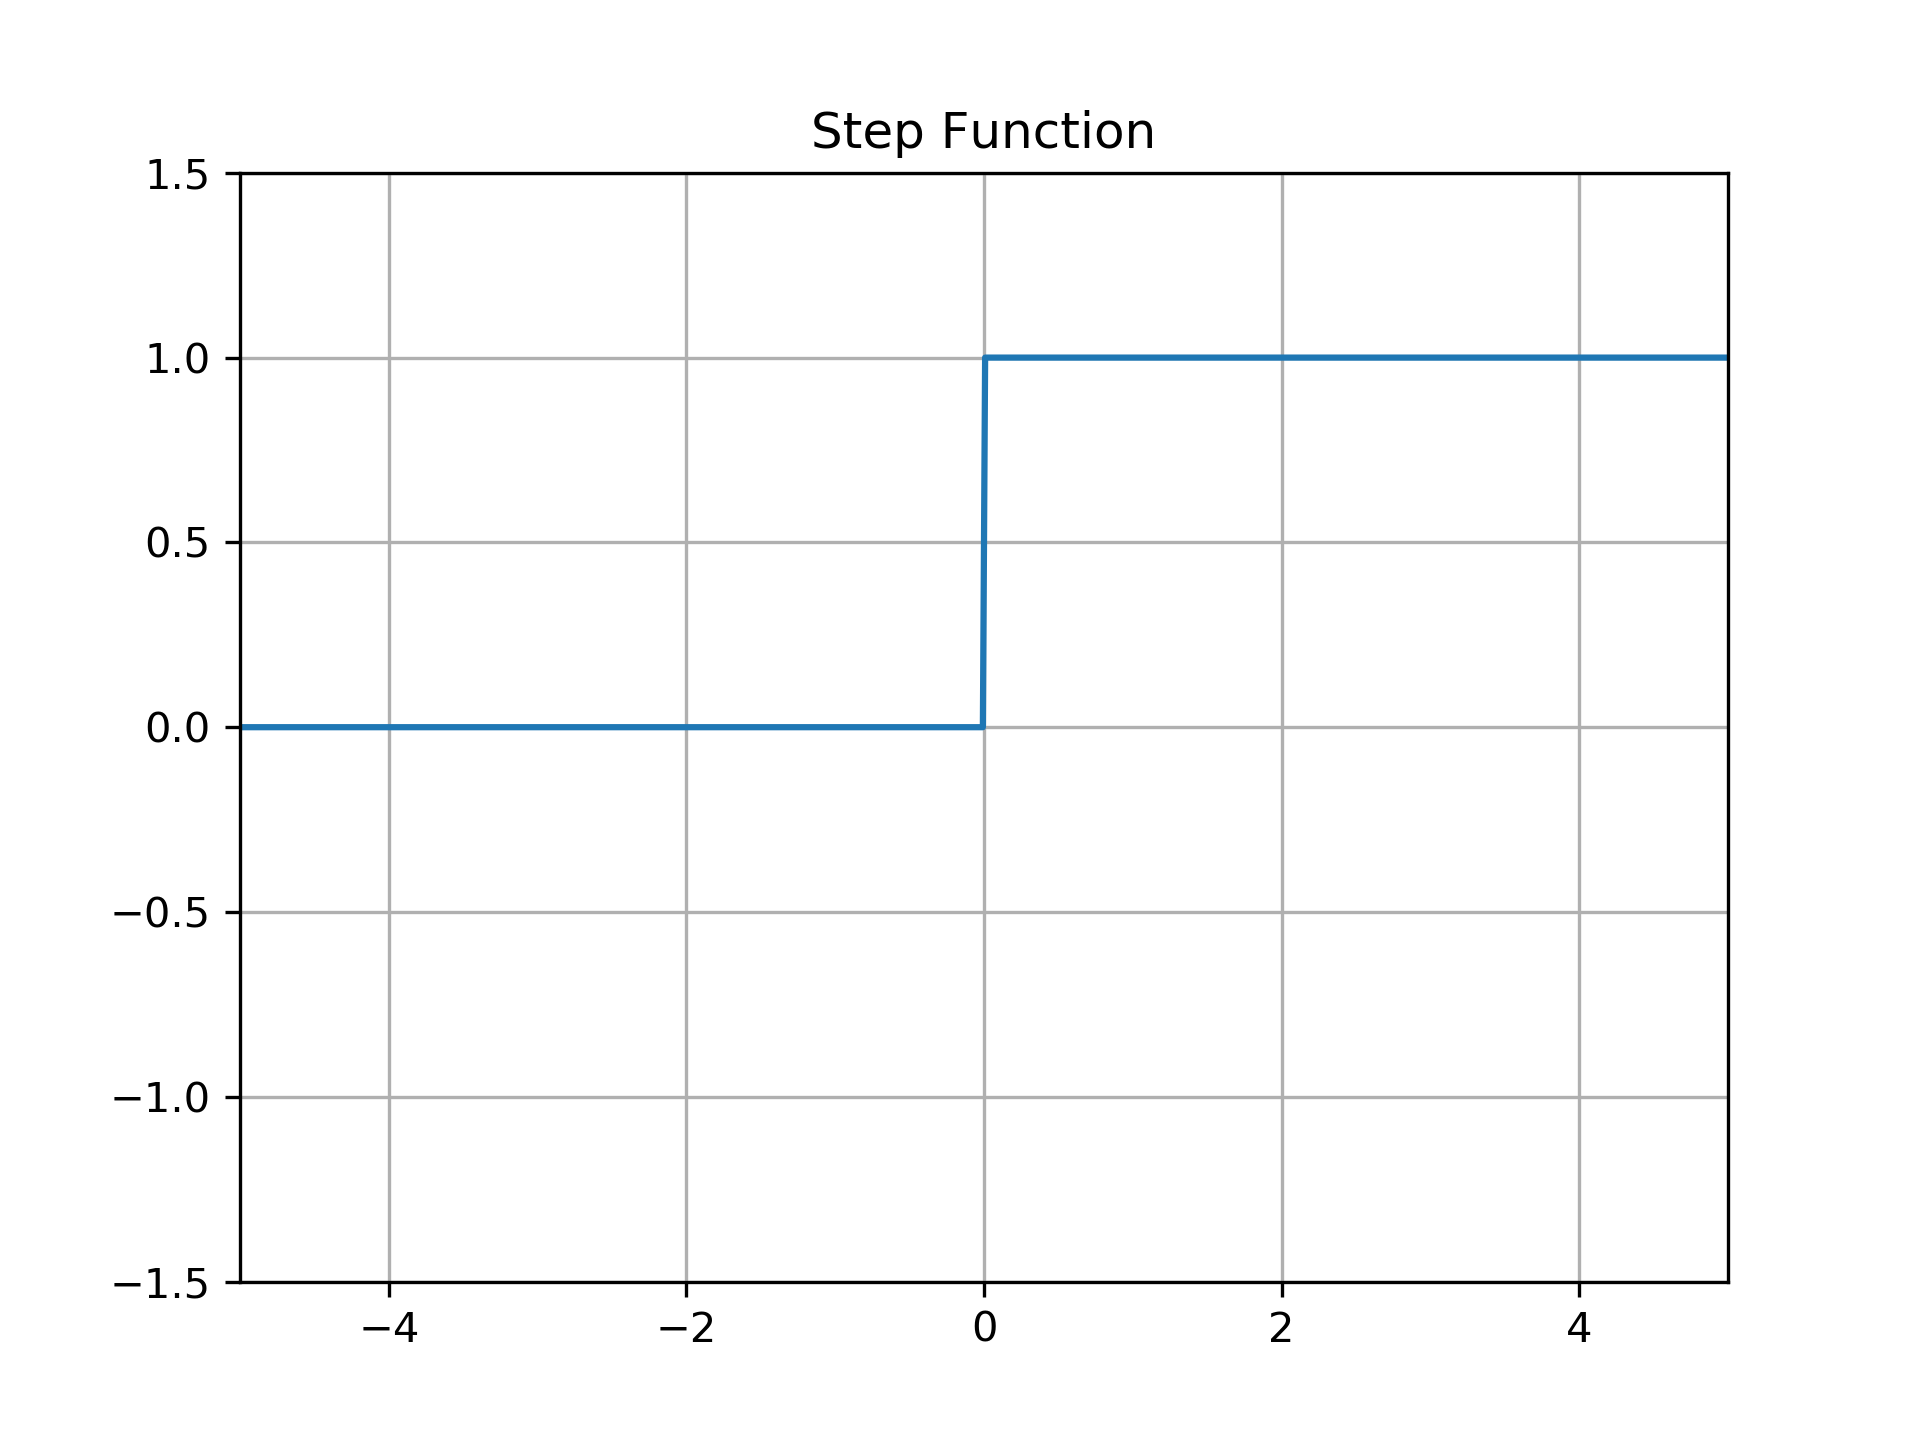
\includegraphics[clip, height=5cm]{figures/deeplearning/af_Step.png}  &
  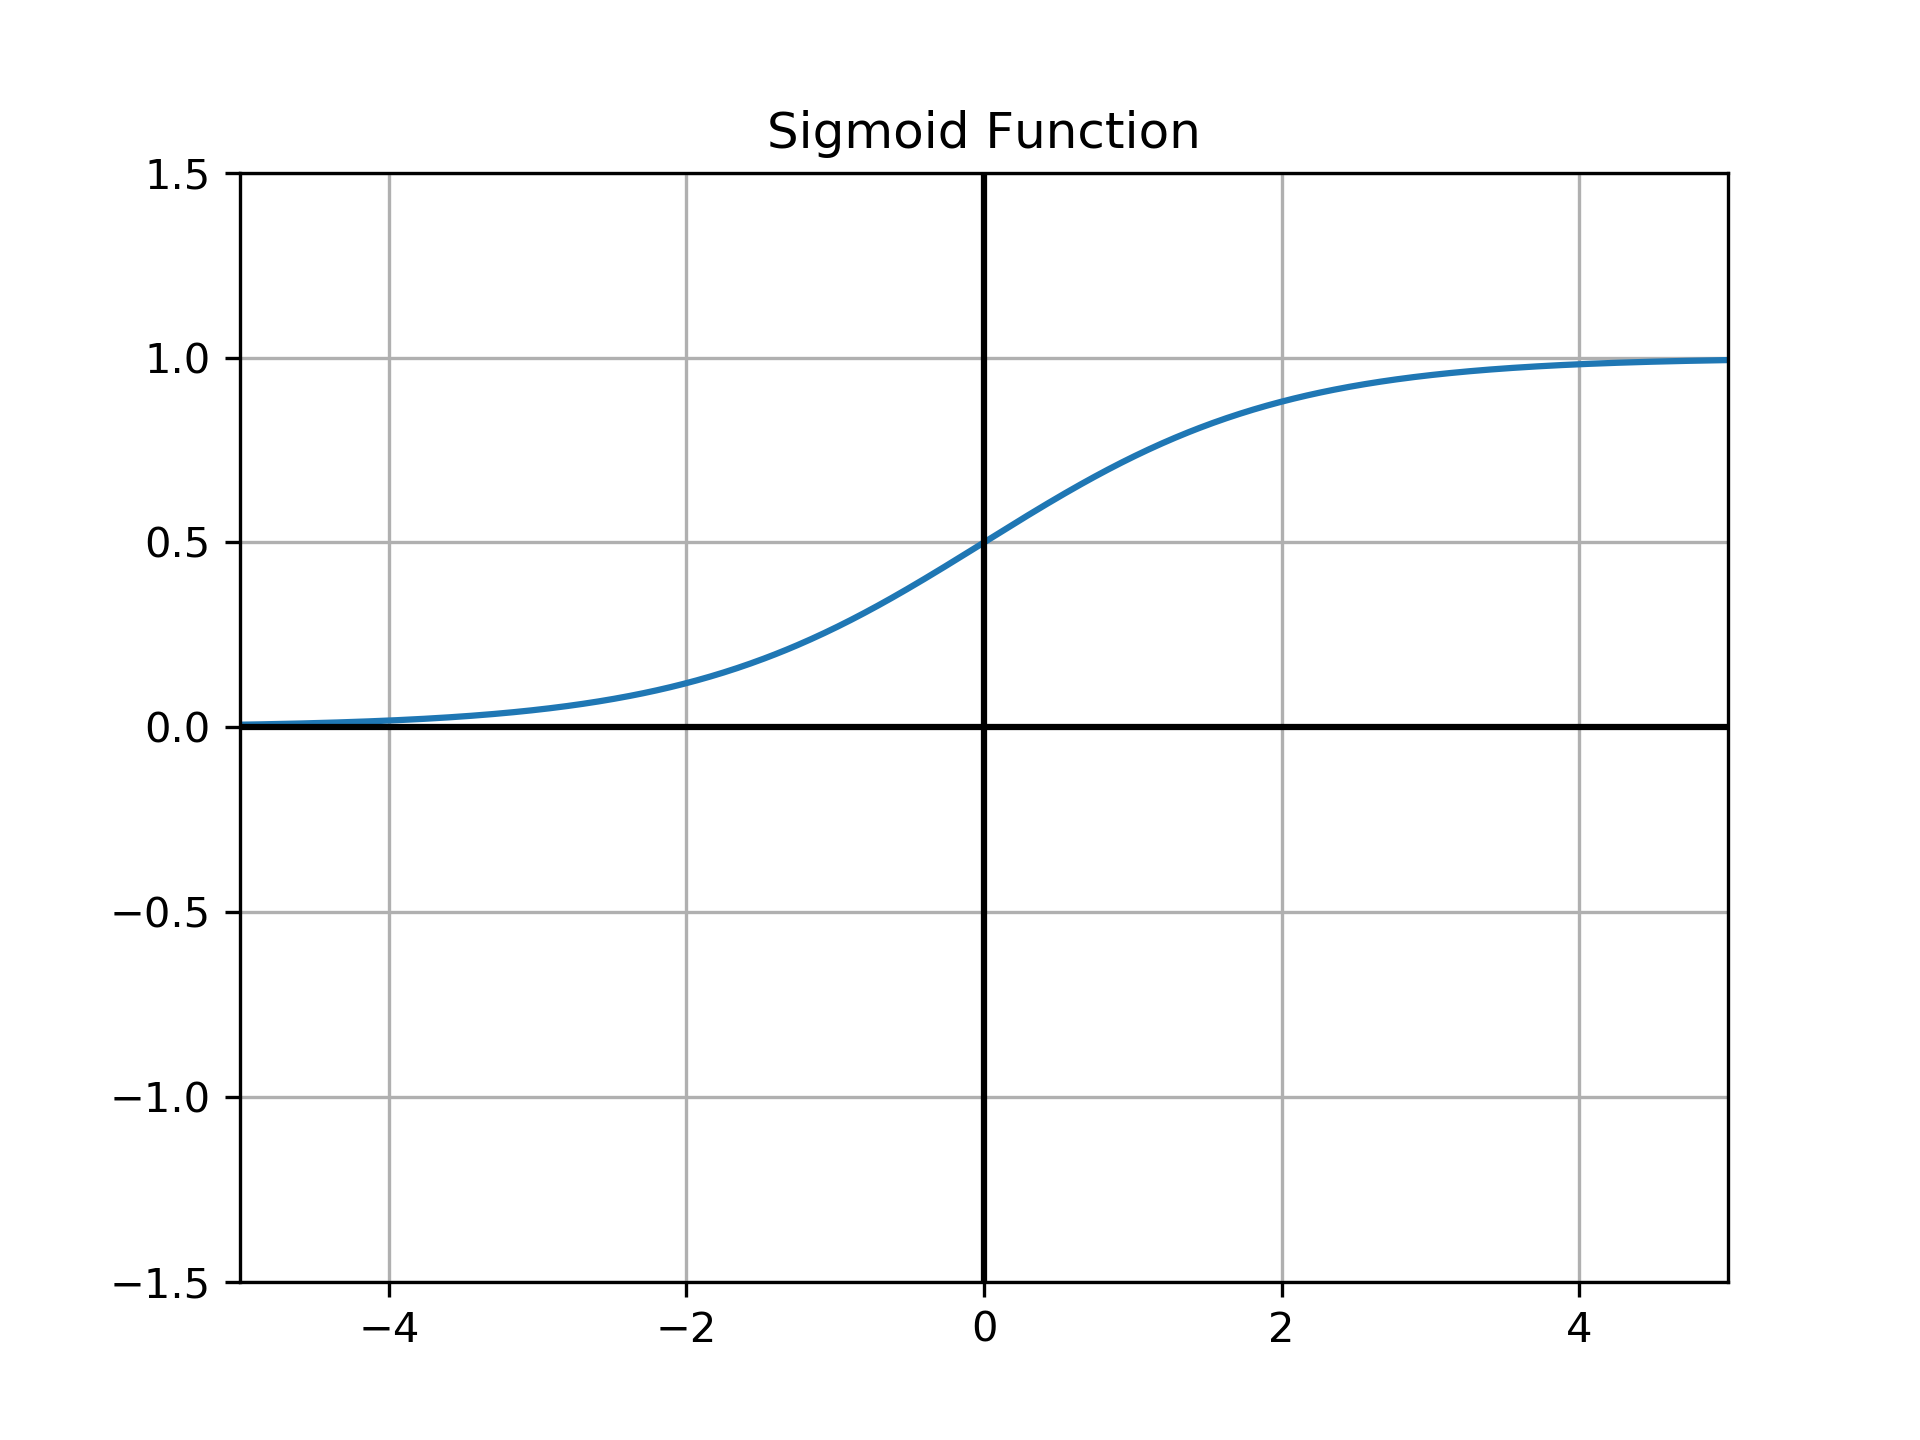
\includegraphics[clip, height=5cm]{figures/deeplearning/af_Sigmoid.png} \\
  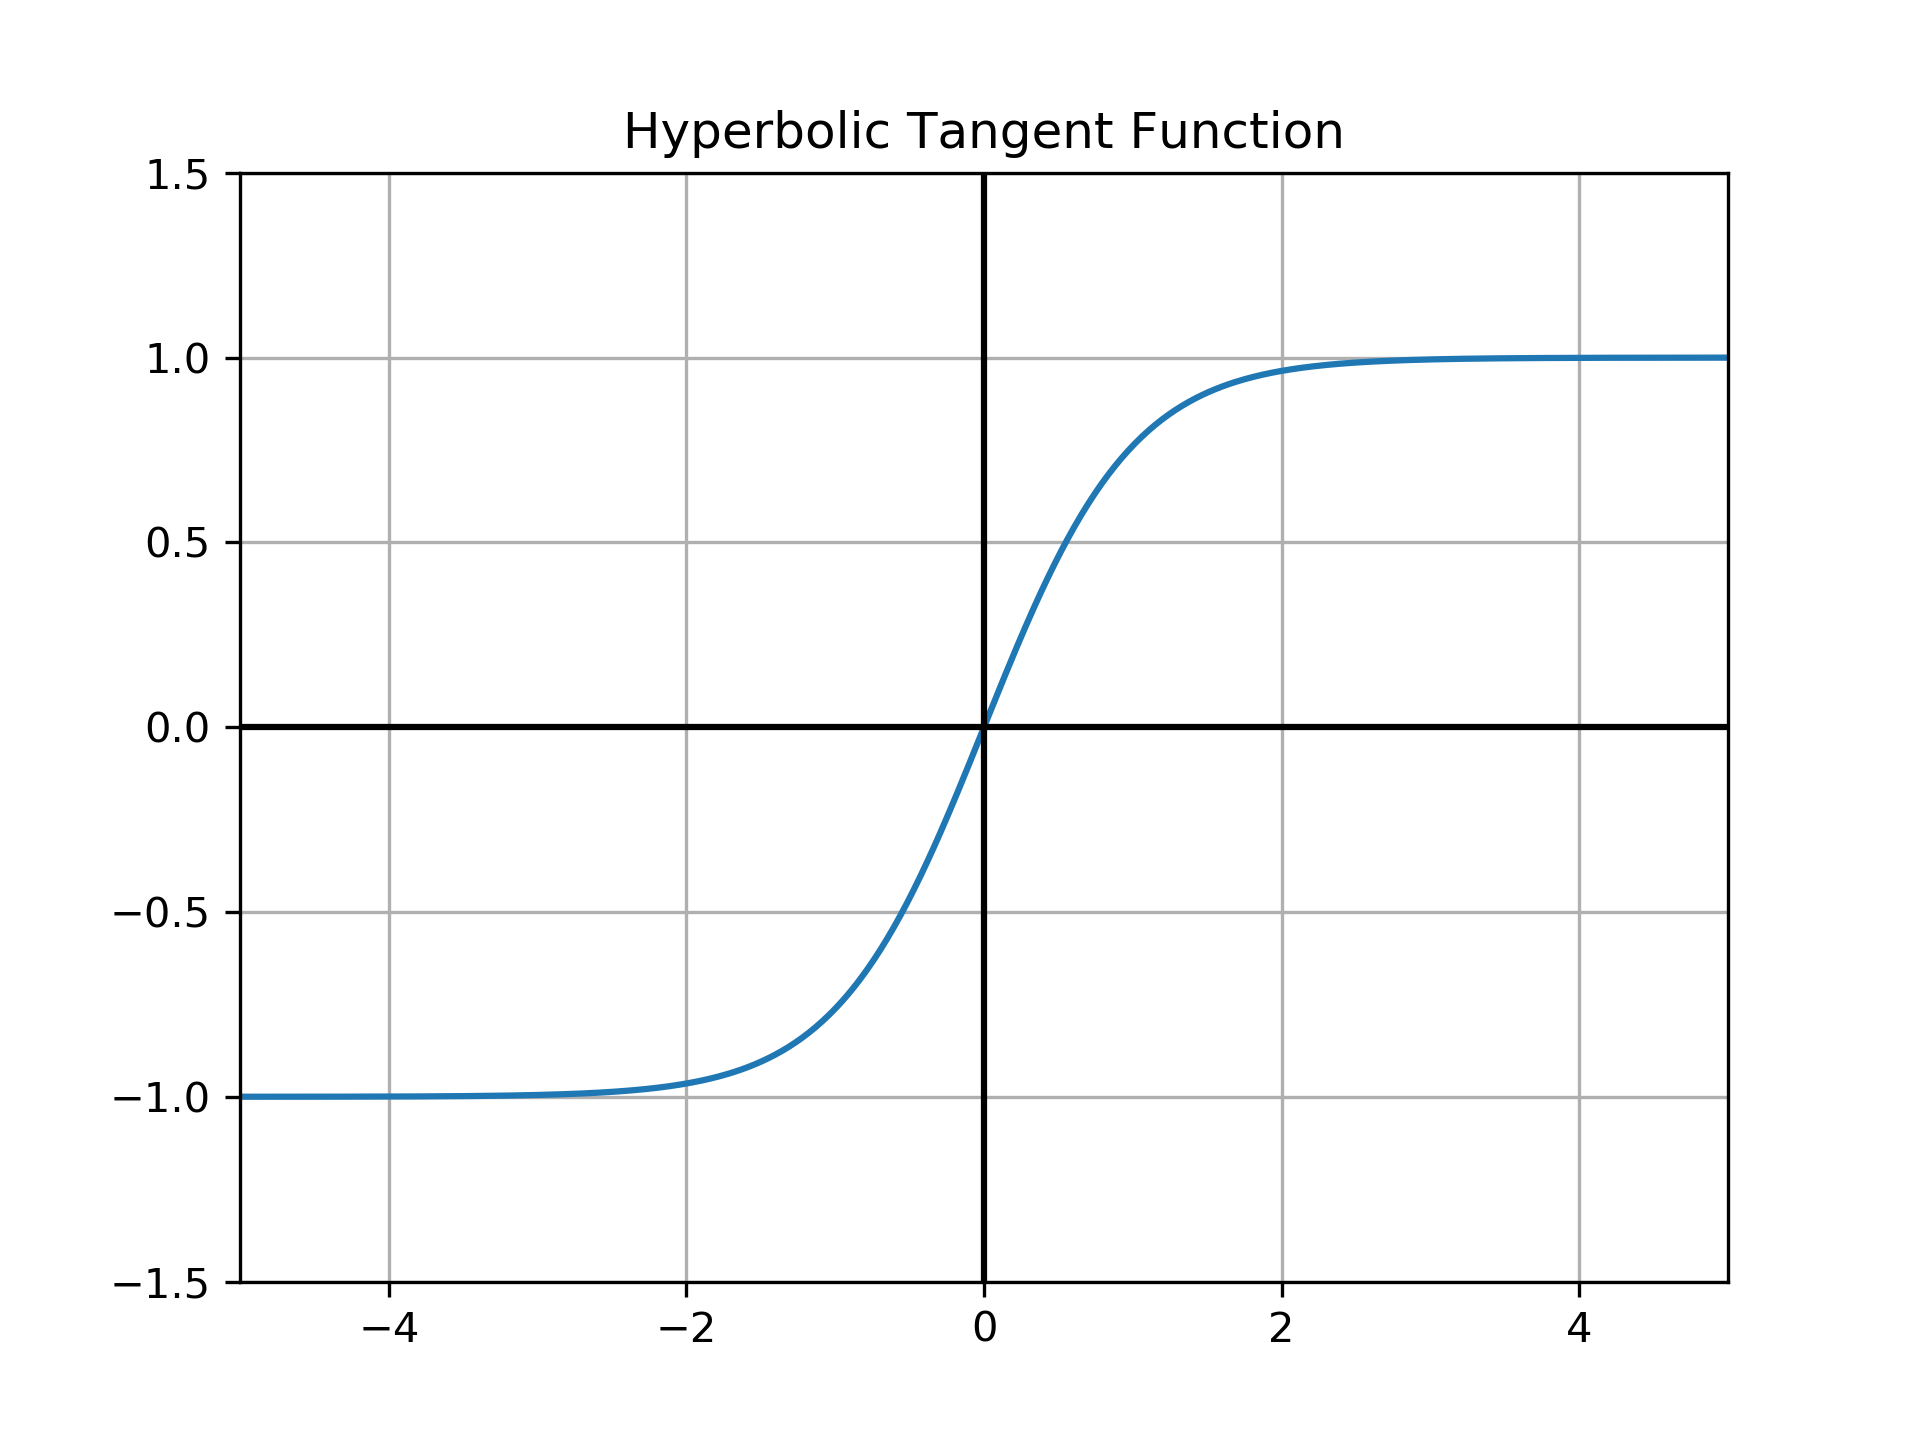
\includegraphics[clip, height=5cm]{figures/deeplearning/af_Hyperbolic.png} &
  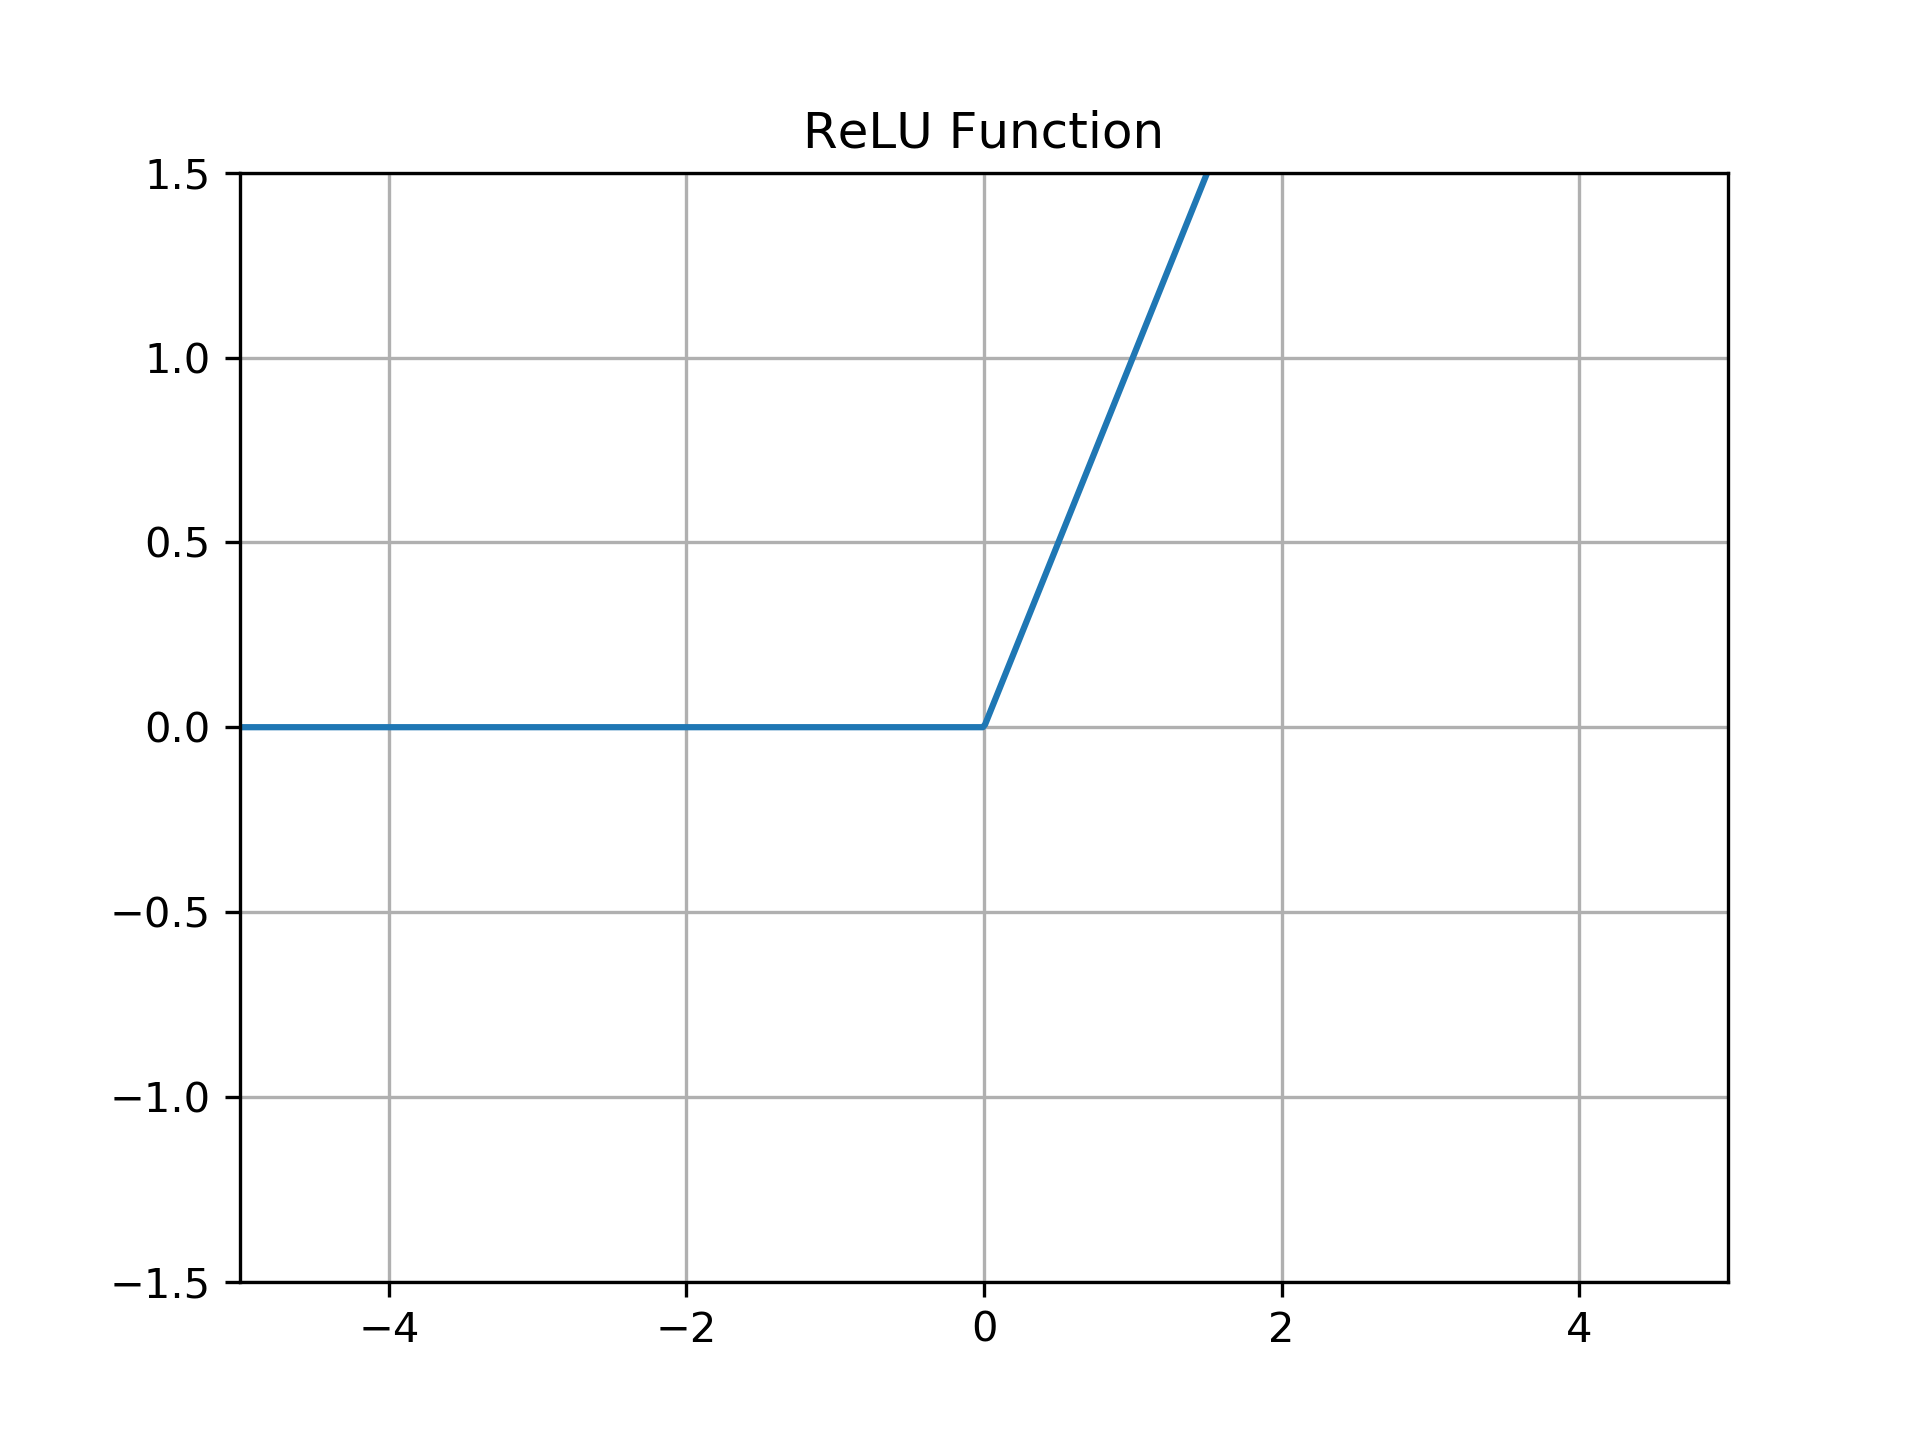
\includegraphics[clip, height=5cm]{figures/deeplearning/af_ReLU.png}  \\
  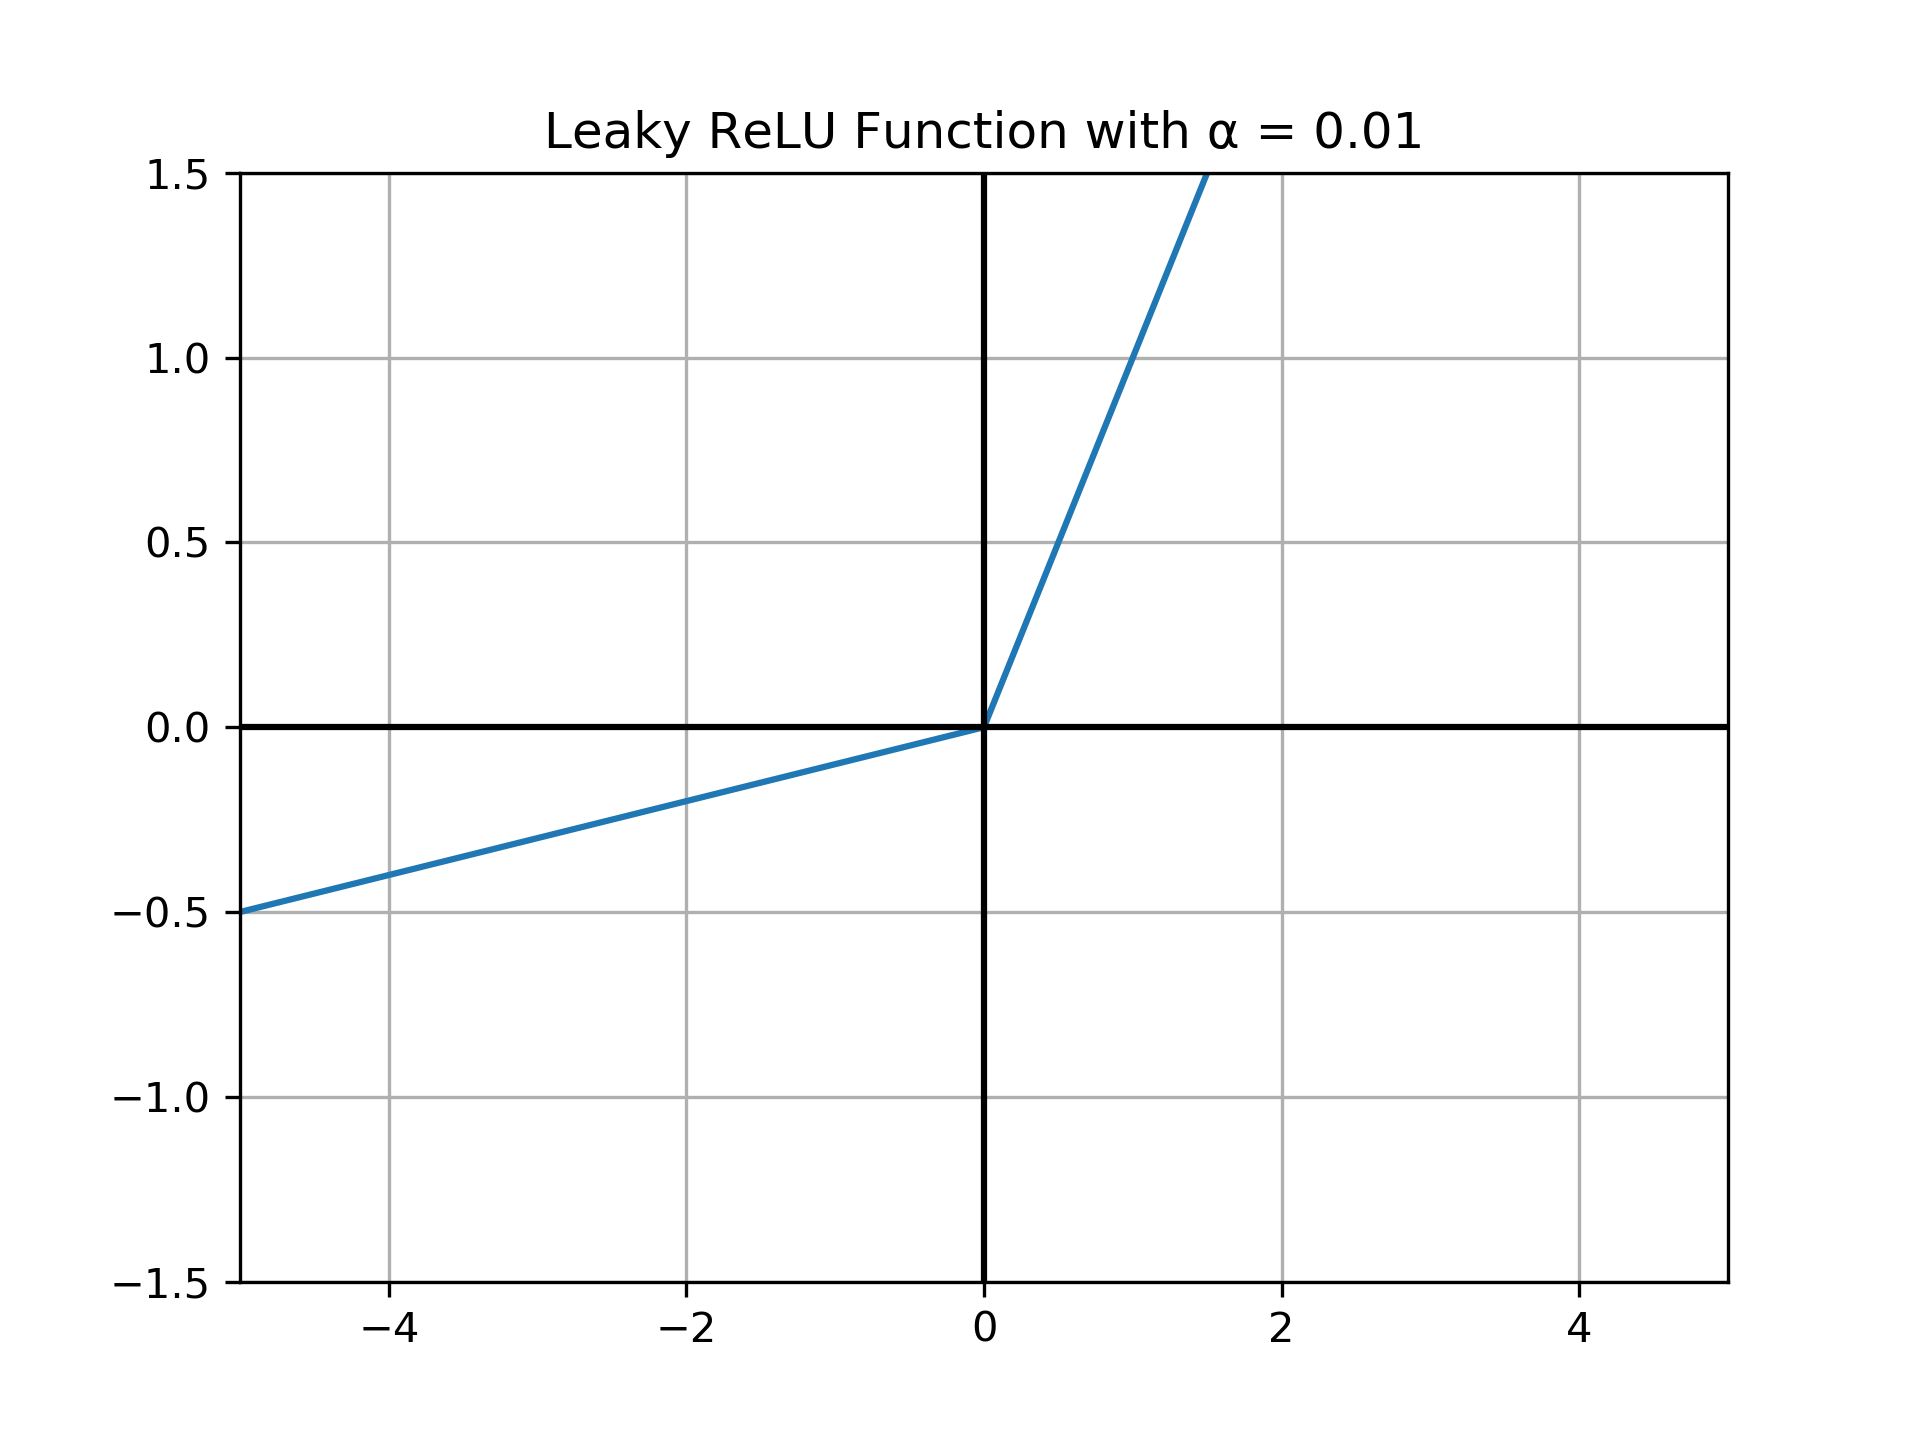
\includegraphics[clip, height=5cm]{figures/deeplearning/af_LeakyReLU.png} & 
  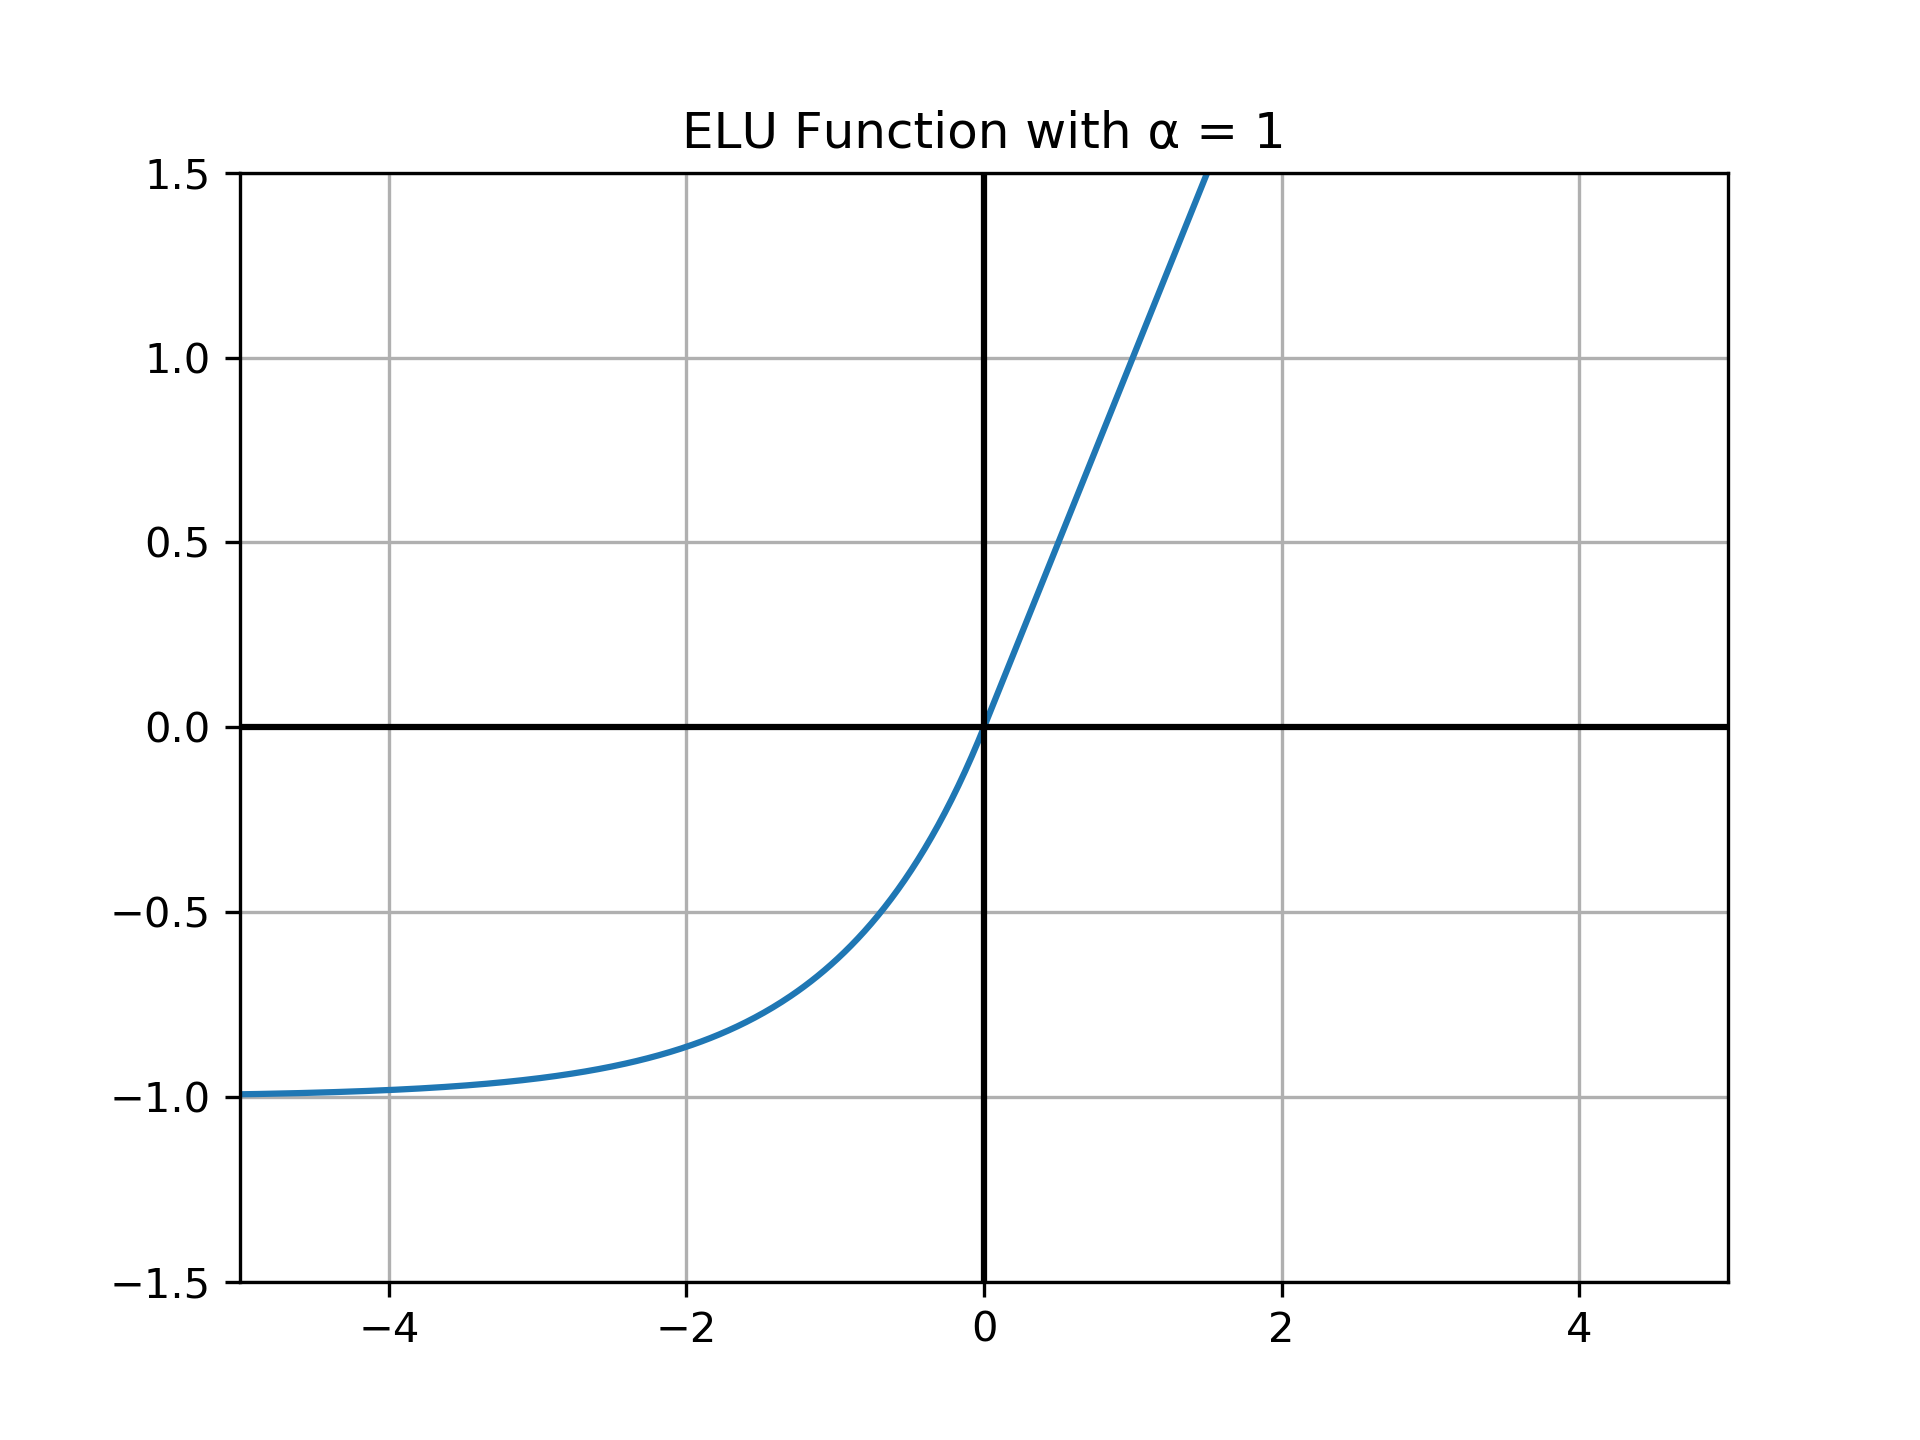
\includegraphics[clip, height=5cm]{figures/deeplearning/af_ELU.png} \\
  
  \end{tabular}
  }%
  \end{center}
  %\vspace*{-12pt}
  \caption[Activation Functions]{Common activation functions. The step function is the only function which cannot be used with the backpropagation algorithm.}
  \label{fig:ActivationFunctions}
  %\vspace*{-12pt}
\end{figure}

\begin{enumerate}
  \item The \textit{sigmoid function} $\sigma(z) = \frac{1}{1 + \exp(-z)}$ \\
    The sigmoid function was originally proposed as a replacement for the step function. It is S shaped and can express values between 0 and 1. It also is continuous, so it has a well-defined nonzero derivate everywhere, while being still similar to the step function in terms of output values.
  \item The \textit{hyperbolic tangent function} $tanh(z) = 2\sigma(2z) - 1$ \\
    The hyperbolic tangent function is similar to the sigmoid function, but its values range from $-1$ to $1$, so layer outputs are centered around 0 at the beginning of the training which speeds up convergence. However it was shown, that bounding the value of the activation function for large $z$ reduces convergence speed.
  \item The \textit{rectified linear unit function} $ReLU(z) = max(0, z)$ \\
    The ReLU function is not differentiable at $z=0$ and has a zero derivate for $z < 0$. Both these properties are not ideal, but the ReLU function is very fast to compute and still performs reasonably well in practice. It is also unbounded in terms of $z$ which further improves convergence. This makes the ReLU function one of the most used activation functions today.
  \item The \textit{leaky rectified linear unit function} $LeakyReLU_\alpha(z) = max(\alpha z, z)$ \\
    One problem with the ReLU function is, that when the weighted sum of the inputs of a neuron is negative for all training instances, the neuron itself will never output anything other than 0 again - the neuron essentially dies. To prevent this the leaky ReLU function has a leak which makes the derivate of the function nonzero for $z < 0$ and prevents the neuron from never learning anything again. The parameter $\alpha$ controls how large the leak should be and can also be learned at training time \cite{xu2015empirical}.
  \item The \textit{exponential linear unit function}
  
  \[ELU_\alpha = 
  \begin{cases} 
    \alpha(\exp(z) - 1) & \text{if } z < 0 \\
    z  & \text{if } z \geq 0
  \end{cases} \]

  Just like the Leaky ReLU function, the ELU function has a nonzero gradient for $z < 0$. If $\alpha = 1$ the ELU function is smooth everywhere. Therefore the ELU function performs better than the Leaky ReLU function, but it is harder to compute. \cite{clevert2015fast} There also exists an extension called SELU which stands for \textit{scaled exponential linear unit} \cite{klambauer2017self} and results in network layers which include self-normalization and therefore preserve a mean of 1 and a standard deviation of 0 during training. This further speeds up training and also showed to improve the results at test time.
  
\end{enumerate}

\subsection{Challenges} \label{sec:NNChallenges}
We saw how we can build neural networks and how they can be trained using gradient descent. Problems - like handwritten recognition - which were extremely complicated for a long time can now be solved with learned models. While in theory we now have the tools to build and train networks, in reality we would quickly encounter problems with networks which just do not learn what we want them to learn. In this Section we want to present some of the most common problems when training neural networks, while also looking at techniques used to avoid them.

\paragraph{Slow Convergence.}
While gradient descent is guaranteed to converge to some minimum if the learning rate is sufficiently small, it makes no guarantees of how much time this convergence process might need. Our simple gradient descent algorithm is only dependent on the first derivate and therefore only "looks" at the slope for the current point. This produces two major problems: If we are on a flat spot of the optimization surface, the gradients will be very small, slowing down training in an "uninteresting" area. The second problem is that always going into the direction of the steepest descent is not the fastest way to the minimum. Instead we would need to additionally look at the second derivate to determine which direction would be optimal. 

To reduce the influence of these problems, a variety of techniques were developed over the years. The basic idea is, that the learning rate does not necessarily have to be a constant, instead we change the step size for each step of gradient descent dynamically depending on the curvature of the optimization surface. For flat regions we could increase the learning rate to compensate for the smaller gradients and lower the learning rate if we detect unstable learning. Directly calculating second derivates has shown to be computationally too expensive. Instead algorithms try to make assumptions about the surface by looking at past gradients. An example of these methods is the idea of \textit{momentum}. 

The momentum method was also proposed by Rumelhart et al. in their backpropagation paper \cite{rumelhart1986learning}. The name originates from real physical momentum, where we think of a particle which is accelerated by a force in a direction. For gradient descent the idea is, that successive gradients usually point in roughly the same direction. Therefore we could improve convergence speed, by just applying the same gradient multiple times. To avoid overshooting, at each step we remember the gradient and compute the new gradient as a linear combination: 
    \[\Delta w = \eta \Delta w - \alpha \nabla f(x_k)\]

Momentum helps to reduce oscillation and is better at avoiding local minima, since the learning process now has the possibility to go over small "hills" in the optimization surface.

The momentum method can easily combined with a second idea: \textit{Learning rate schedules}. Picking an initial learning rate that is optimal for the whole learning process is hard. Initially we will be far from the optimum and need a higher learning rate to converge faster and avoid local minima and over time, the training process might get closer to the optimum but begin to oscillate around it, because the learning rate is too high. To always work with an optimal learning rate, we need to adjust it over time and these strategies are the learning schedules. Some often used schedules are:

\begin{enumerate}
  \item \textit{Linear Scheduling}. The easiest schedule is a linear schedule where the learning rate is a function of $\eta(t) = \eta_0 - (\eta_0 * t/s)$. The effective learning rate is linearly annealed from a starting learning rate $\eta_0$ to zero. The parameter $s$ is set to be the total number of training steps for SGD.
  \item \textit{Power Scheduling}. The learning rate is a function of the form $\eta(t) = \eta_0 / (1 + t/s)^c$ with the hyperparameters $c$ - the exponent - and $s$ - the number of steps. With power scheduling, the learning rate will decrease every $s$ steps, arriving at $\eta_0 / 2$ after $s$ steps, $\eta_0 / 3$ after $2s$ steps and so on. This results in an effective learning rate which quickly drops and then decreases more and more slowly over the course of training.
  \item \textit{Exponential Scheduling}. The learning rate is a function of $\eta(t) = \eta_0 \cdot 0.1^{t/s}$. The learning rate will therefore drop by a factor of 10 every $s$ steps.
  \item \textit{Performance Scheduling}. Measure the validation error every $N$ steps and reduce the learning rate by a factor $\gamma$ when the error did not drop. 
\end{enumerate}

There also exist a lot of other schedules like piecewise scheduling, where the learning rate is defined for specific parts of the training process. The choice of the learning rate schedule is dependent on the task and also influence by other factors like overfitting.

Since the learning rate is the most important hyperparameter for deep learning over the years many other more sophisticated methods were developed, most notable \textit{AdaGrad} \cite{duchi2011adaptive}, \textit{RMSProp} \cite{tieleman2012lecture} and \textit{Adam} \cite{kingma2014adam} which are usually used in nowadays neural network frameworks. All these algorithms use the past gradients to calculate per-parameter learning rates based on a given starting learning rate. They often make use of momentum optimization and can be used in conjunction with learning rate schedules.


\paragraph{Overfitting.}
\textit{Overfitting} is a recurring problem for all machine learning techniques. When training on a training dataset, we expect the trained model to have the same performance on new never seen before data. To achieve this, our goal is to learn a representation of our input data. The problem arises when the model is too closely fit to the training dataset, which often happens if our model has too many parameters and if we trained our model too long. Overfitted models often show an extremely low training error of close to 0\%, while on test time  the model performs very bad. Overfitted models usually did not learn a representation of the data, but instead just "remember" each sample from the training dataset. We therefore also speak about models which fail to generalize. An example for overfitting in a classification task is given in Figure \ref{fig:Overfitting}. We can see, that the overfitted model did not ignore the noise in the training data and instead created a decision boundary which perfectly separates both classes in the training dataset, but does not model the true distribution behind the data.

\begin{figure}[ht]
  
  \begin{center}
    \resizebox{0.95\columnwidth}{!}{%
    \begin{tabular}{ccc}
    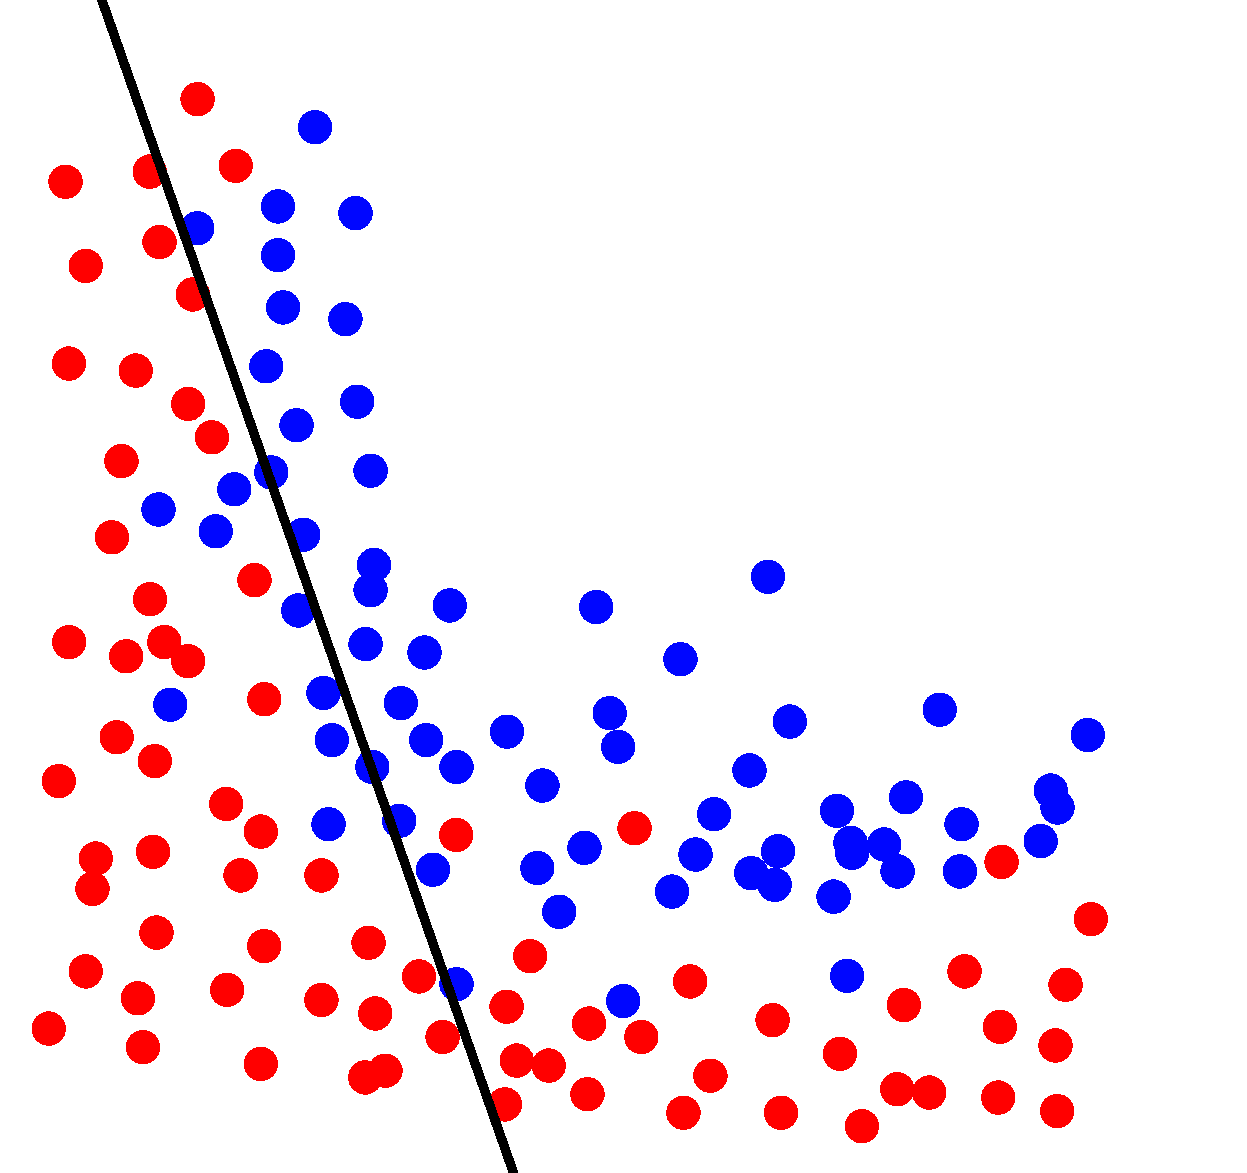
\includegraphics[clip, height=5cm]{figures/deeplearning/Underfitting.pdf}  &
    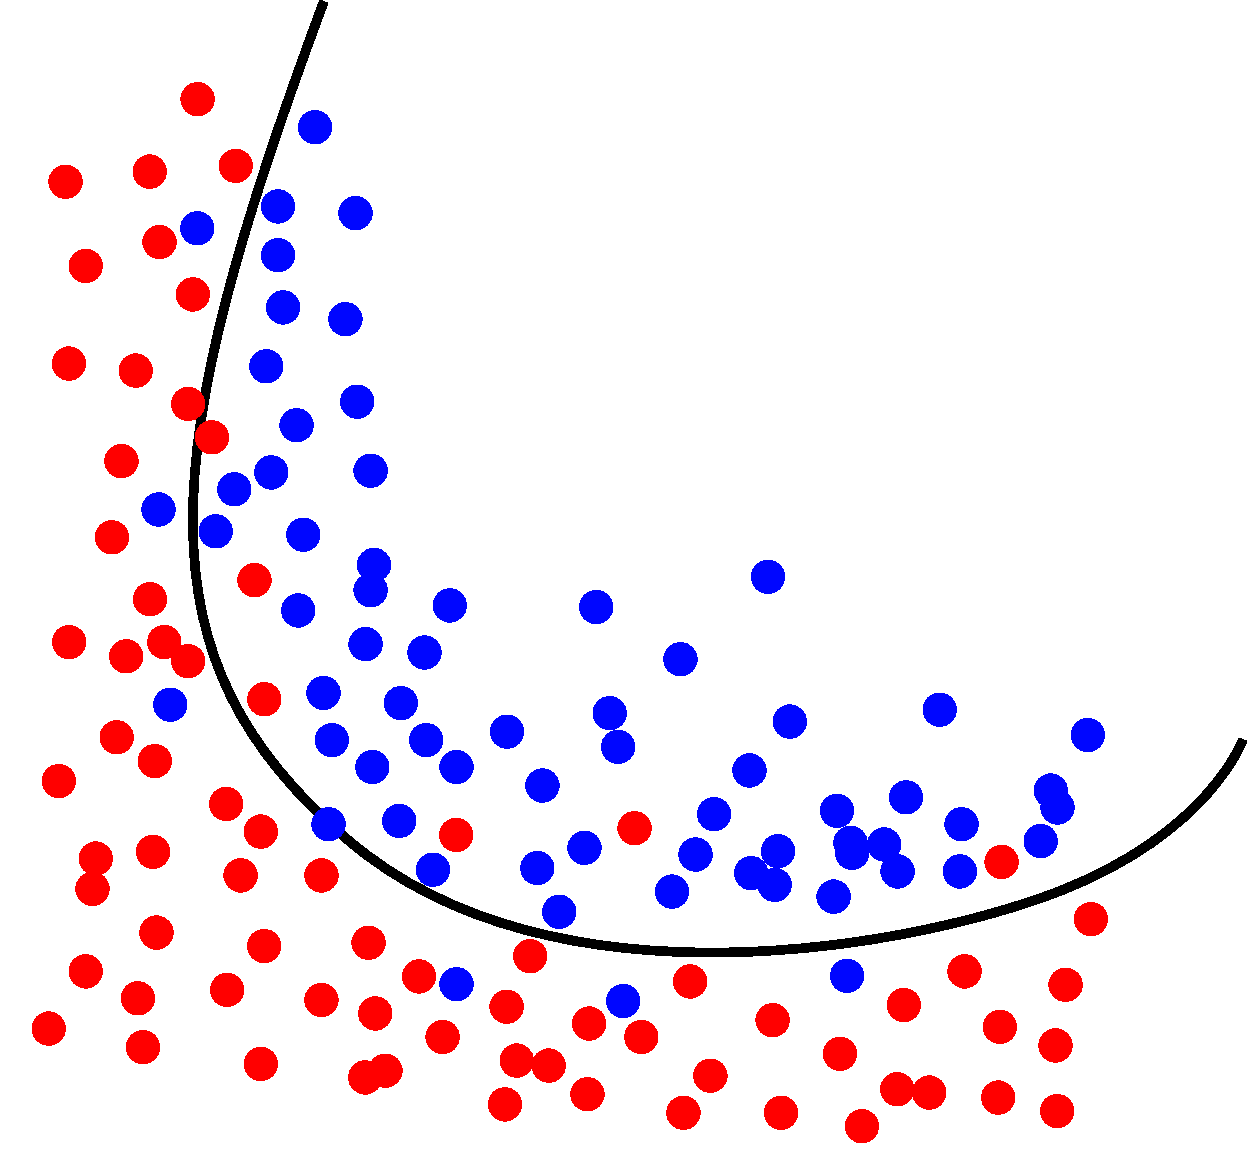
\includegraphics[clip, height=5cm]{figures/deeplearning/IdealModel.pdf} & 
    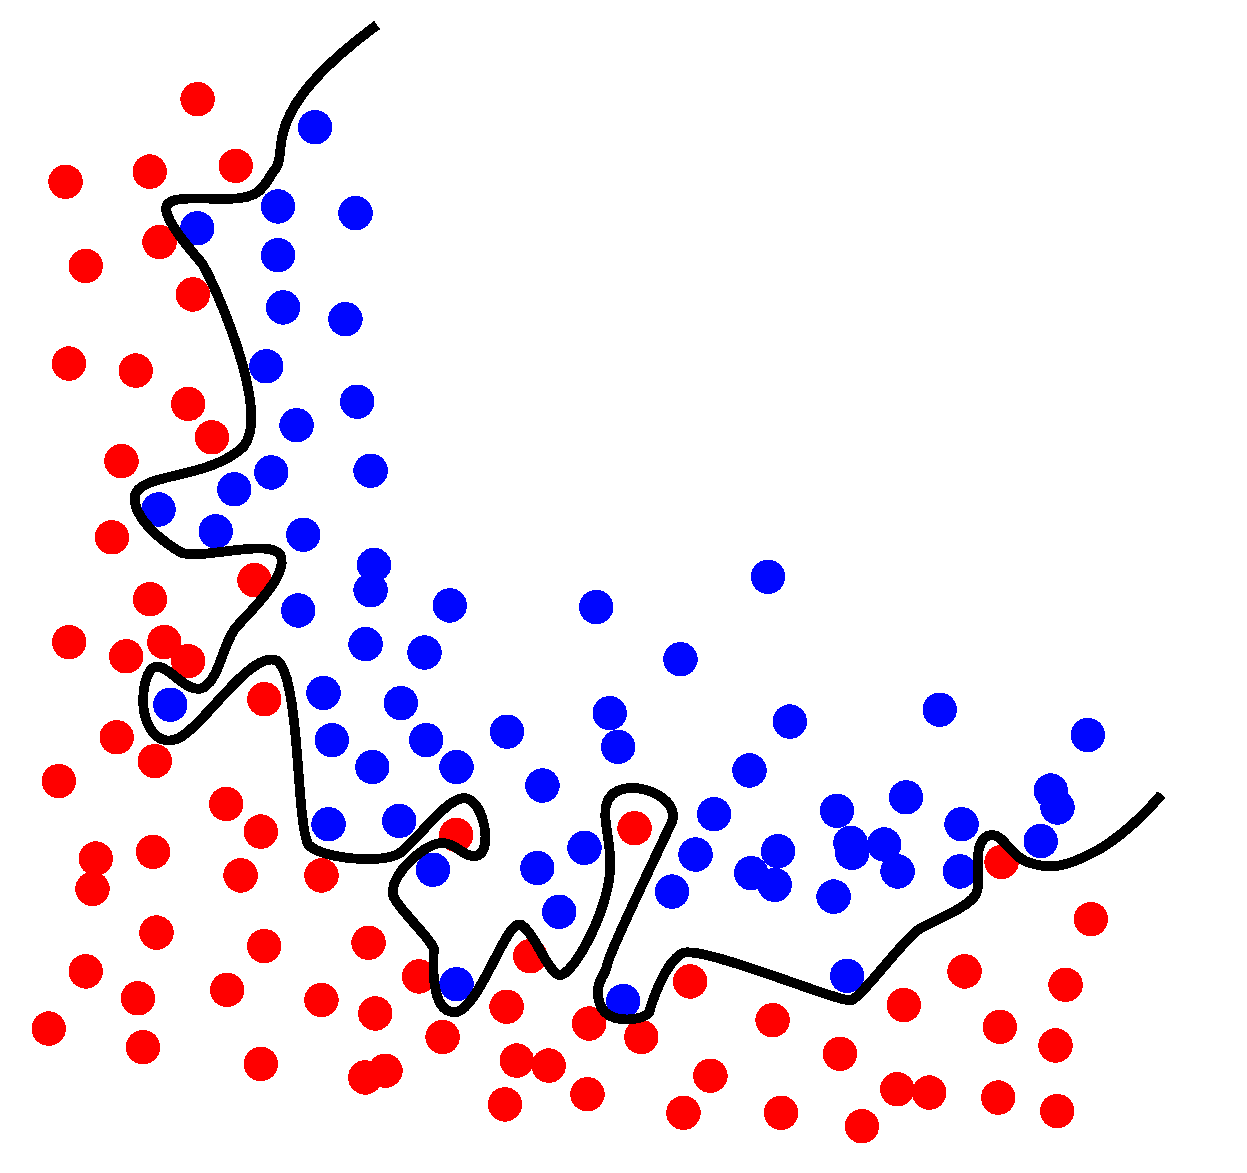
\includegraphics[clip, height=5cm]{figures/deeplearning/Overfitting.pdf}\\
    {Underfitting} &
    {Perfect Model} &
    {Overfitting} \\
    
    \end{tabular}
    }%
    \end{center}
  
  %\vspace*{-6pt}
  \caption[Overfitting Example]{This example demonstrates the effects of over- and underfitting for a 2-dimensional dataset with samples of two classes blue and red. We can see, that neither the underfitted nor the overfitted models will work well on test data, even though the overfitted model will have a 0\% error rate on the training dataset.\footnotemark}
  \label{fig:Overfitting}
  %\vspace*{-12pt}
\end{figure}

\footnotetext{Original image created by user Ignacio Icke, released under Creative Commons under \url{https://commons.wikimedia.org/wiki/File:Overfitting.svg}, edited and extend with underfitting example.}

Neural networks generally have a high tendency to overfit on the training data, because their size and the resulting number of parameters enables the network to very closely fit to the training data. When training, it usually makes sense to create a balance between the number of samples we have to train the network and the number of parameters (neurons) inside of our network. If we do not have much training data we need a smaller neural network to avoid overfitting too quickly. Overfitting is also influenced by the learning rate. If the learning rate is high enough, gradient descent will never converge completely and the network will therefore generalize better. Therefore the danger of overfitting increases when using advanced optimizers or learning rate scheduling to adapt the learning rate dynamically.

Luckily there are better ways of preventing overfitting than using a high learning rate or not use advanced optimizers. In the following we present a number of methods, which can be used in conjunction to prevent or detect overfitting.

\begin{enumerate}
  \item \textit{Early Stopping}. Before we start the training process, we can split our training data into two datasets - a training and a validation dataset. When training the neural network, we periodically test the performance of the model on the validation dataset. If the model did not improve for a certain amount of time on the validation dataset (or even gets worse) we stop training to avoid overfitting. Early stopping is very effective and easy to implement, but requires to split the training data which results in less training data for the learning process.  
  \item \textit{Regularization}. One of the best ways to prevent overfitting is to use regularization methods to keep the weights of the neural network from getting too large. To achieve this a regularization term is added to the loss function. There are three widely used methods:
  \begin{itemize}
    \item $l_2$ regularization from \textit{Ridge Regression} (also called \textit{Tikhonov} regularization) can be used to explicitly punish single large weights in the network. To achieve this a regularization term is added to the loss function which adds a weight penalty according to the $l_2$ norm:

      \[\mathcal{L}_{l_2} = \frac{\gamma}{2} \sum_{i=1}^n \theta^2_i \]

      The sum starts at $i=1$, because the bias term is usually not regularized. There also exists an alternative idea of how to implement $l_2$ regularization called \textit{weight decay} which just multiplies each weight with a constant $c < 1$ after each training step.
    
    \item $l_1$ regularization from \textit{Lasso Regression}. $l_1$ regularization also adds a term to the loss function, but this time the $l_1$ norm is used so the weights contribute equally. 

      \[\mathcal{L}_{l_1} = \gamma \sum_{i=1}^n |\theta_i| \]

      An interesting characteristic of the $l_1$ regularization is that it produces weights close to zero for the least important features. This produces a sparse model where many connections will have a zeroed out weight.
    
    \item \textit{Max-Norm Regularization} is another regularization technique which simply limits the $l_2$ norm of the connection weights $\mathbf{w}$ to a certain value, such that $|| \mathbf{w} ||_2 \leq r$. Max-Norm regularization can be implemented similar to weight decay by rescaling the weights after each training step to $\mathbf{w} \leftarrow \mathbf{w} r/||\mathbf{w}||_2$ if needed. 

  \end{itemize}
  
  \item \textit{Dropout}. Dropout is one of the latest regularization techniques which was proposed in 2012 by Hinton et al. \cite{hinton2012improving}. At each training step, every neuron (excluding output neurons) has a probability of $p$ to be ignored ("dropped out") during the current training step. The probability is usually set surprisingly high to values between 10\% and 50\%. While being simple to implement, dropout is not only a powerful regularization technique, but also makes the network more robust. 
  
  You can think about dropout in an interesting way: Since every neuron has a chance to be dropped out or be present at each training step, a network with dropout essentially represents $2^N$ distinct networks at once. The resulting network during test is composed out of all these smaller networks building a strong ensemble classifier. Neurons in the network are also less likely to co-adapt, making the network less error prone for slight input changes like noise at test time and improving overall generalization.  
\end{enumerate}



\paragraph{The Unstable Gradients Problem.}
When we talked about the backpropagation algorithm in Section \ref{sec:Backpropagation} we stated, that it is possible to train arbitrary neural networks with it, regardless of the number of layers. While this is true to some extend the backpropagation algorithm initially struggled to train networks with more than three layers. Since the gradients are computed layer-wise and propagated backwards from the outputs to the inputs using the connection weights, the gradient between the layers $i$ and $j$ (meaning layer $i$ is the input layer to layer $j$) shrinks or grows depending on 

\[F_{i,j} = ||\phi(v_j) \cdot \mathbf{w}_{i, j}||_1\]

This means, that if $F_{i, j} < 1$ the gradients tend to get exponentially smaller for each layer which is called the \textit{vanishing gradients problem} and if $F_{i, j} > 1$ the gradients tend to exponentially grow which is called the \textit{exploding gradients problem}. Both problems lead to networks, which contain upper layers which do not learn anything and are therefore often worse in performance than networks with less layers.

To prevent the gradients from exploding or vanishing, we need to look at both, the activation function and the weights. As for most problems, there are multiple solutions which can be used standalone or in conjunction with others, to enable the BP algorithm to properly work for deep neural networks:

\begin{enumerate}
  \item \textit{Non-Saturating Activation Functions.} We already presented a number of activation functions in Section \ref{ssec:ActivationFunctions}. The initially used sigmoid activation function had two crucial problems for its application in deep neural network. First, its slope is at most 0.25, which means errors in backpropagation always tend to get smaller with each layer. Second, the function saturates to 0 and 1 for very small or very large inputs, leading to very small gradients at these points and thus very slow learning. The solution is to use one of the other activation functions which do not saturate to a maximum value. Therefore deep neural networks usually use either ReLU, Leaky ReLU, ELU or SELU activations. 
  \item \textit{Improved Network Weight Initialization.} In 2010 Glorot and Bengio proposed a way to deal with unstable gradients, by using a new method to initialize the weights \cite{glorot2010understanding}. Usually weights in neural networks were randomly initialized with a normal distribution with a mean of 0 and a standard deviation of 1. Glorot and Bengio showed, that for backpropagation we need to control the variance of the outputs of each layer in both directions - for the forward pass and for the backpropagation. This means, that the output distribution of each layer should have equal variance to the input distribution and at the same time we need the variance of the gradients needs to be the same before and after each layer. Completely satisfying this constraint is only possible if two adjacent layers have the same number of neurons, but the initialization can still be optimized. If we denote the number of input neurons by $fan_{in}$, the number of output neurons by $fan_{out}$ and the average number by $fan_{avg} = (fan_{in} + fan_{out}) / 2$, the Glorot initialization is given by 

  \begin{align*}
    &\text{A normal distribution with mean 0 and variance } \sigma^2 = \frac{1}{fan_{avg}} \\
    &\text{Or a uniform distribution between -r and +r, with } r = \sqrt{\frac{3}{fan_{avg}}}
  \end{align*}
  
  This initialization strategy has proven to successfully minimize effects of the unstable gradients problem at the beginning of training. Depending on the used activation function, the initialization strategy needs to be adapted slightly. ReLU and ELU activation functions use the so-called He initialization with $\sigma^2 = 2 / fan_{in}$ and the SELU activation function uses the LeCun initialization with $\sigma^2 = 1 / fan_{in}$.
  \item \textit{Batch Normalization.} The problem with a good initialization of the network is, that the problem is only prevented from appearing directly at the start of the training process. Therefore in 2015 Ioffe and Szegedy proposed to a new techniques called \textit{Batch Normalization} (BN) to keep the output of each layer normalized with respect to some distribution. Their algorithm adds an additional operation before (or after) the activation function of each layer to zero-center, scale and shift the input for each layer. The parameters for the shift and scaling operations are learned at training time by computing an average over the current minibatch (therefore the name \textit{batch} normalization). The input for each layer can then be calculated in four steps:


  \begin{enumerate}\setcounter{enumii}{0}\renewcommand\theenumii{\arabic{enumii}}
    \item Calculate the mean input vector over the minibatch $B$: $\displaystyle \mu_B = \frac{1}{m_B} \sum_{i=1}^{m_B} x^i$ 
    \item Calculate the standard deviation over the minibatch $B$: $\displaystyle \sigma_B^2 = \frac{1}{m_B} \sum_{i=1}^{m_B} \left(x^i - \mu_B\right)^2$
    \item Calculate zero-centered and normalized input vectors: $\displaystyle \hat{x}^i = \frac{x^i - \mu_B}{\sqrt{\sigma_B^2 + \epsilon}}$
    \item Calculate rescaled and shifted outputs: $\displaystyle z^i = \gamma \otimes \hat{x}^i + \beta$
  \end{enumerate}
  
  The scaling parameter $\gamma$ and the shift parameter $\beta$ are learned via backpropagation together with the other variables of the neural network. Because $\mu_B$ and $\sigma_B$ are only calculated for the current batch, it is not ideal to use them at test time. Instead they are usually calculated by either recalculating them over the whole training dataset, or to calculate them at training time by using a running mean. Batch normalization significantly improves the performance of deep neural networks, but adds additional complexity at both training and test time.
  \item \textit{Gradient Clipping.} To avoid overhead like in batch normalization, an easy way to deal with exploding gradients is to just clip the value of the gradients to be in a certain range, e.g in $[-1, +1]$. This was first used by Razan et al. in 2013 for the training of recurrent neural networks, which are complicated to combine with batch normalization \cite{pascanu2013difficulty}. To keep the direction of the gradient it is also possible to clip by normalizing the gradient vector to the $l_2$ norm.
  \item \textit{Residual Networks.} Another take on the unstable gradients problem is the use of residual neural networks. These networks contain skip connections (shortcuts) which directly feed the output of one layer to another layer which is not its direct successor. Figure \ref{fig:ResidualBlock} shows a residual building block for a network. 
  
  \begin{figure}[t]
    
    \begin{center}
        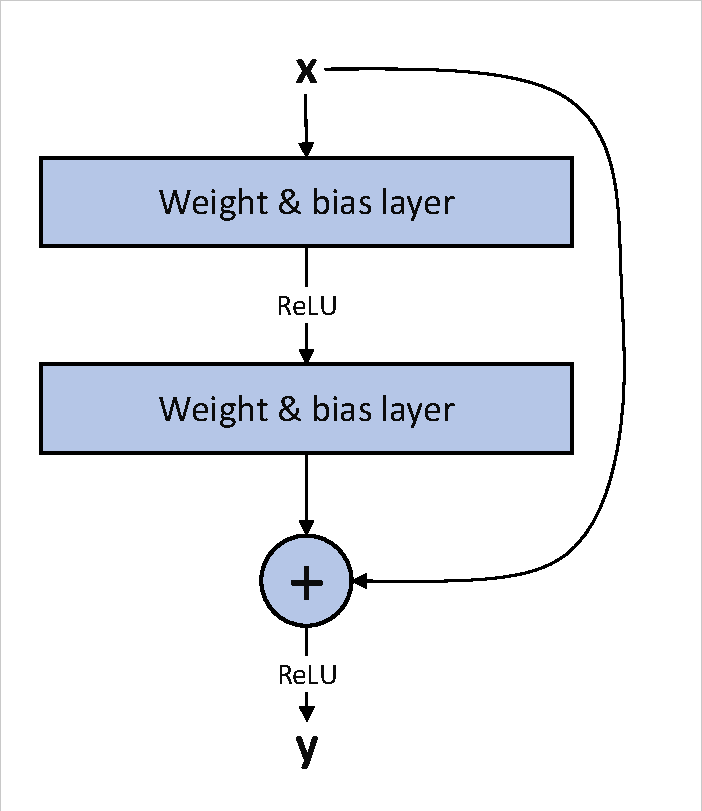
\includegraphics[clip, trim=10px 10px 10px 10px, width=0.4\columnwidth]{figures/deeplearning/Residual_Block.pdf}
    \end{center}
    
    %\vspace*{-6pt}
    \caption[Residual Block]{The structure of a residual block. Deep neural networks without skip connections are not able to learn the identity for a layer when trained with BP. Therefore larger networks often perform worse than shallower ones. With skip connections, networks can learn deviations from the identity, which works far better and also eliminates unstable gradients.}
    \label{fig:ResidualBlock}
    %\vspace*{-12pt}
  \end{figure}

  Skip connections are motivated by biological structures in the cerebral cortex. In 2016 Xu et al. first used residual connections in artificial neural networks for image recognition \cite{he2016deep}. They showed, that large networks with residual connections are faster to train and yield better end results without batch normalization. By skipping layers, the network is able to propagate errors from the output directly into layers close to the input of the network, allowing networks which have hundreds of layers. Having lower level features at later stages of deep networks also seems to be beneficial for the overall performance.
\end{enumerate}

\section{Specialized Network Structures} \label{sec:SpecializedNetworks}
Until now we only were working with fully connected feed forward networks. While every fully connected layer is able to model any other arbitrary connection with the next layer, it is faster to train networks which already contain a certain structure, if that structure directly benefits the task. Especially image recognition has shown to be hard, even for larger multilayer networks. Therefore a special architecture is used when dealing with pixel inputs which we will explore in Section \ref{ssec:CNNs}. Sometimes we are also confronted with continuous input data which requires memory. To deal with time dependent input data, another special network architecture exists, which we will take a look at in Section \ref{ssec:RNNs}. 

\subsection{Recurrent Neural Networks} \label{ssec:RNNs}
Feed forward neural networks are great for making predictions on data without a time component, e.g. images classification tasks. But if you want to predict the future, you often need to remember the past. And that is one thing our networks are missing: A memory. Think of a self-driving car, which has to keep track of all its surroundings. A pedestrian might walk on the sidewalk and at some point get obscured by a parking car. If we remember that we saw that pedestrian some time ago, we can expect him to suddenly reappear and maybe cross the road. This is especially important if our pedestrian is a child which might not watch out for a car. A normal feed forward network would forget about the child as soon as it can not see it anymore, but if we had some kind of memory we would be able to remember the child and slow down. This situation cannot always be solved by adding timed information as input to the neural network (e.g. having a sequence of images from a video stream as input rather than a single image) as we do not know ahead of time for how long our memory has to last. 

\begin{figure}[ht]
    
  \begin{center}
      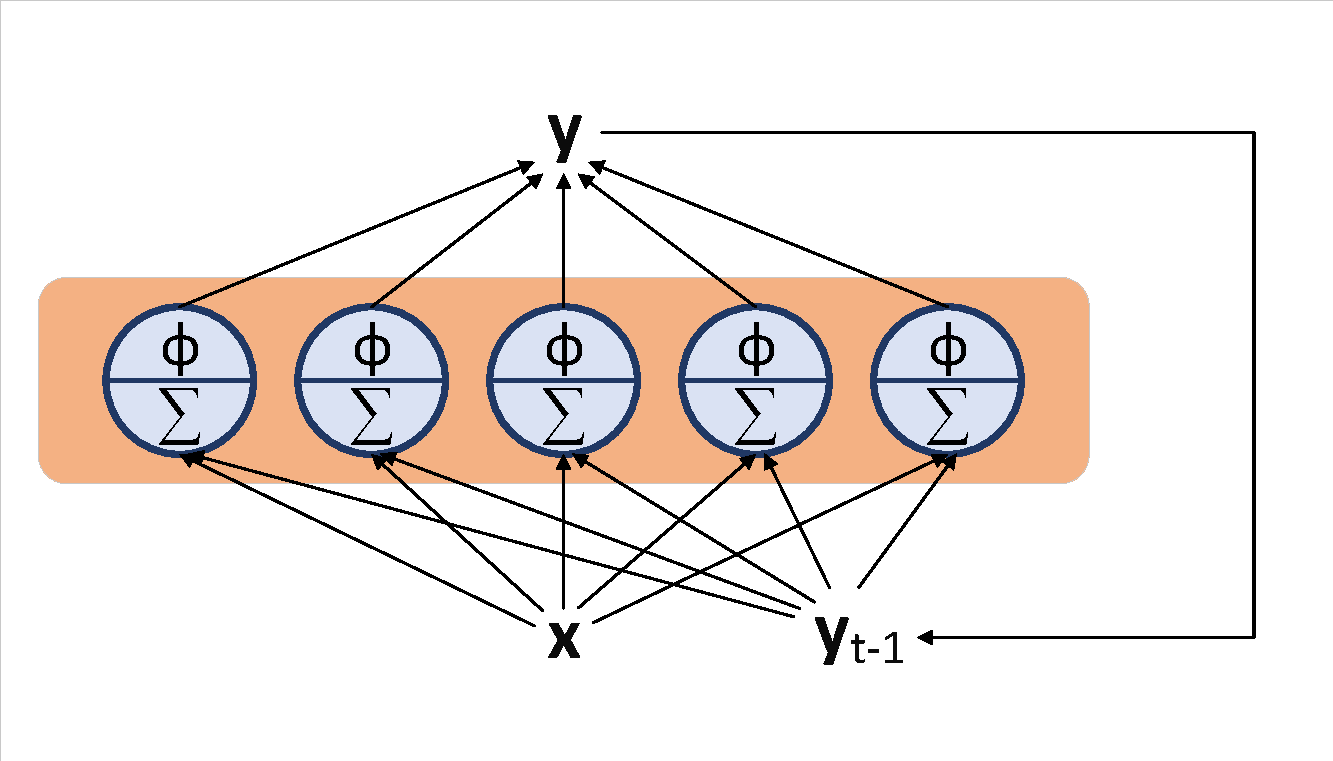
\includegraphics[clip, trim=10px 10px 10px 10px, width=0.7\columnwidth]{figures/deeplearning/Recurrent_Layer.pdf}
  \end{center}
  
  %\vspace*{-6pt}
  \caption[Recurrent Layer]{A layer in a recurrent neural network. The output $\mathbf{y}$ of the layer is used as a input for the next timestep.}
  \label{fig:RecurrentLayer}
  %\vspace*{-12pt}
\end{figure}

To solve this problem, we modify the neurons of our network. Instead of having only a single flow direction from the input to the output, our new network also has connections pointing backwards. This type of network is called a \textit{recurrent neural network} (RNN). Usually each layer of a RNN takes its own output as additional input vector in the next time step. This way, the network is able to remember its past inputs and its decisions at the same time. We included a representation of a recurrent layer in Figure \ref{fig:RecurrentLayer}. At step $t$ each recurrent neuron receives two input vectors: The current input vector $\mathbf{x}_t$ and its own output vector of the previous step $\mathbf{y}_{(t-1)}$. Accordingly each recurrent neuron has two sets of weight vectors $\mathbf{w}_x$ and $ \mathbf{w}_y$. If we look at the whole layer of neurons and their weights $\mathbf{W}_x$ and $\mathbf{W}_y$ we can compute the layer output by 

\[\mathbf{y}_t = \phi(\mathbf{W}_x^T \mathbf{x}_t + \mathbf{W}_y^T \mathbf{y}_{(t-1)} + \mathbf{b})\]

Recurrent neural networks are harder to train than regular feedforward networks, but essentially still rely on classical backpropagation. The trick is to unroll the network through time and then train it using regular backpropagation. This method for training RNNs is called \textit{backpropagation through time} (BPTT). BPTT unrolls the network for a fixed number of timesteps $T$ into the past. The first recurrent vector is set to 0 and the output of each unrolling step is evaluated by a cost function. The gradients of the cost function are then backpropagated through the unrolled network, so the weights and biases are actually updated multiple times for a single learning step. 

Recurrent neural networks can be used for a multitude of tasks which require time series data. They are especially well suited for natural language recognition, processing or translation as well as forecasting of future sequences (e.g. stock market prices) or the processing of video input. Since training of RNNs is hard because the unrolling process produces very deep network structures, often a modern improved version of RNNs called \textit{long short-term memory} (LSTM) is used, which was developed in 1997 by Hochreiter and Schmidhuber \cite{hochreiter1997long}. LSTMs implement a completely new and complex model for a single neuron which allows it to remember information for longer periods of time and be trained more efficiently.


\subsection{Convolutional Neural Networks} \label{ssec:CNNs}
Although many tasks can quickly be solved by standard feedforward neural networks, performing tasks on images proofed to be notoriously hard. While detecting objects in a picture seems to be effortless for humans, machine learning struggles with every aspect of image recogition. But what makes the task so easy for humans and so difficult for machines? Since humans (and most other animals which live on land) rely on their ability to see, they developed a complex preprocessing pipeline which allows them to see, without learning how to see. Before the signals from our eye reach our visual cortex, they are preprocessed and already transformed into high-level features. Our brain therefore never needs to deal directly with the raw signals from our retina. Even though our brain is incredibly powerful, this preprocessing allows it to handle images in a fast and reliable way (well most of the time, since the preprocessing is also responsible for how many optical illusions work). 

In 1958 and 1959 David Hubel and Torsten Wiesel experimented with cats to understand how their visual cortex works \cite{hubel1959single, hubel1959receptive}. They found out, that neurons that are directly connected to the retina only react to local stimuli on a specific region. They also were able to show, that certain neurons only react to images of horizontal lines, while others only react to lines with different orientations. Later neurons then combine these lower level features and only react to complex features build from these lower level patterns. In 1998 LeCun et al. were able to adapt this structure for artificial neural networks in their \textit{LeNet-5} architecture \cite{lecun1998gradient} which is the first \textit{Convolutional Neural Network} (CNN). CNNs introduce two new building blocks which build the foundation of modern image recognition: The \textit{convolutional layer} and the \textit{pooling layer}.

\paragraph{Convolutional Layers.} Convolutional layers resemble their biological counterparts by not being fully connected. Instead each neuron of the convolutional layer is only connected to a small region on its input layer. This means each neuron only reacts to local signals of a specific $n \times m$ region inside of the previous layer. Each additional layer therefore learns higher level features, based on the lower level ones from the previous layer. In Figure \ref{fig:ConvolutionalConnections}, we show an example of a convolutional layer. The neuron in the $i$th row and $j$th column is connected to the neurons of the previous layer in a window with size $f_h \times f_w$ and centered at $(i, j)$. To avoid each layer from getting smaller than the previous one, the layer can be padded with zeros. If the layer instead should reduce the complexity, the windows can be used with a stride $s$ to achieve a downscaling effect. The stride defines how far the window is shifted between two neurons.  

\begin{figure}[ht]
    
  \begin{center}
      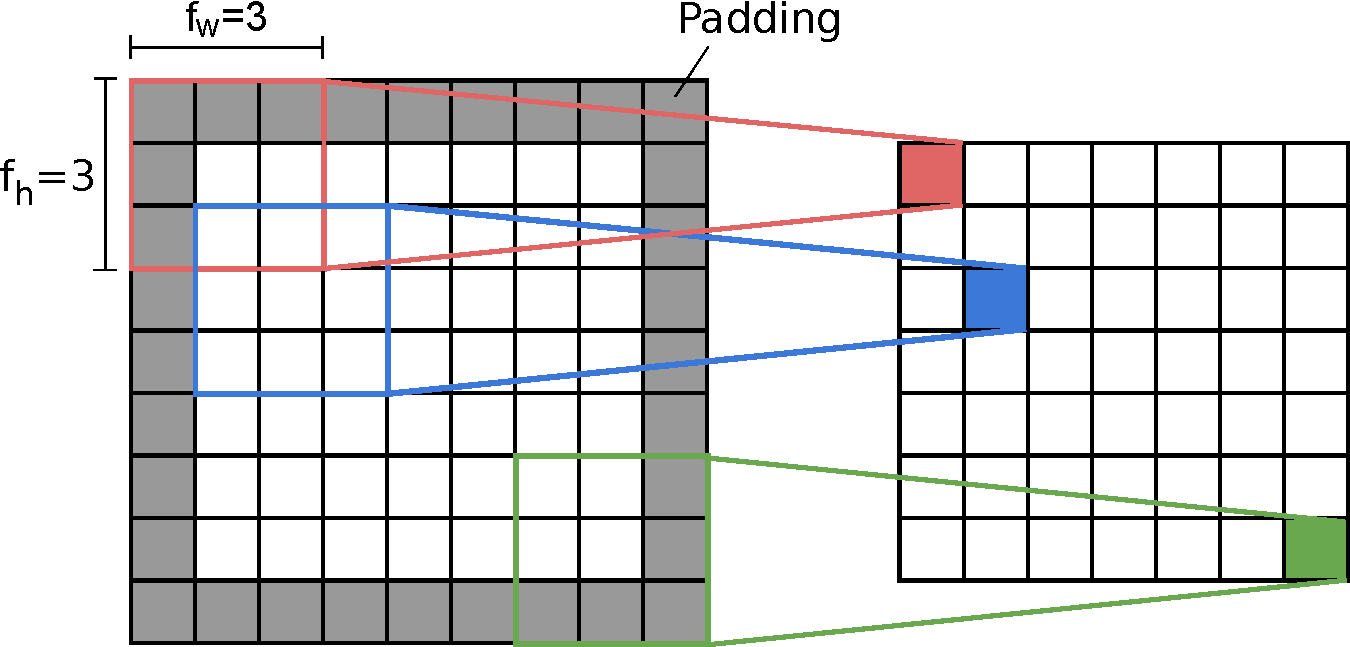
\includegraphics[clip, width=0.7\columnwidth]{figures/deeplearning/Convolution.pdf}
  \end{center}
  
  %\vspace*{-6pt}
  \caption[Convolutional Connections]{Connections in a convolutional layer with a window of $3 \times 3$ and a stride of 1. The input is padded to avoid downscaling. Neurons are only connected locally with rectangular receptive fields.}
  \label{fig:ConvolutionalConnections}
  %\vspace*{-12pt}
\end{figure}

An important idea when using convolutional networks is, that a feature that is interesting in one area (e.g. horizontal lines) may also be interesting in every other area of the input image. We call the neurons whose weights compute a specific feature a \textit{filter} or \textit{kernels}. If we use the same weights and biases of the filter for the whole layer (called \textit{weight tying}), the output of the layer is a \textit{feature map}. This feature map contains the output of a filter placed at every position at the previous layer. To allow the network to learn multiple filters, a layer in a convolutional network is a stack of feature maps generated by multiple filters. Each feature map is connected to the full depth of all feature maps of the previous layer. For example if we have an $100 \times 100$ RGB image (3 channel input) and construct $20$ filters with size $5\times 5$, every neuron of the first convolutional layer will be connected to $5\times 5 \times 3 = 75$ input neurons. The layer then will output 20 images of size $100 \times 100$ as output, one for each filter. Filters of size $5\times 5$ of a second convolutional layer will therefore work on a input size of $5\times 5 \times 20 = 500$ values.

The fact that each filter only needs to be trained once while being able to use it on every part of the input image produces a large advantage compared to fully connected layers. Its internal structure allows the CNN to vastly reduce the number of parameters needed to express a filter operation over the complete image. The only downside is, that a CNN produces large intermediate results, because each filter outputs a complete copy of the image which needs a lot of memory.

\paragraph{Pooling Layers.} Pooling layers work similar to convolutional layers only on a local part of the input, but serve a different function. Pooling layers \textit{subsample} (i.e. shrink) the input. We already saw, that our intermediate results get pretty large, so by downscaling them, we are able to save computational resources, reduce memory usage and also reduce the numer of parameters (which prevents overfitting). Pooling layers also introduce invariance against small translations in the input image. 

\begin{figure}[ht]
    
  \begin{center}
      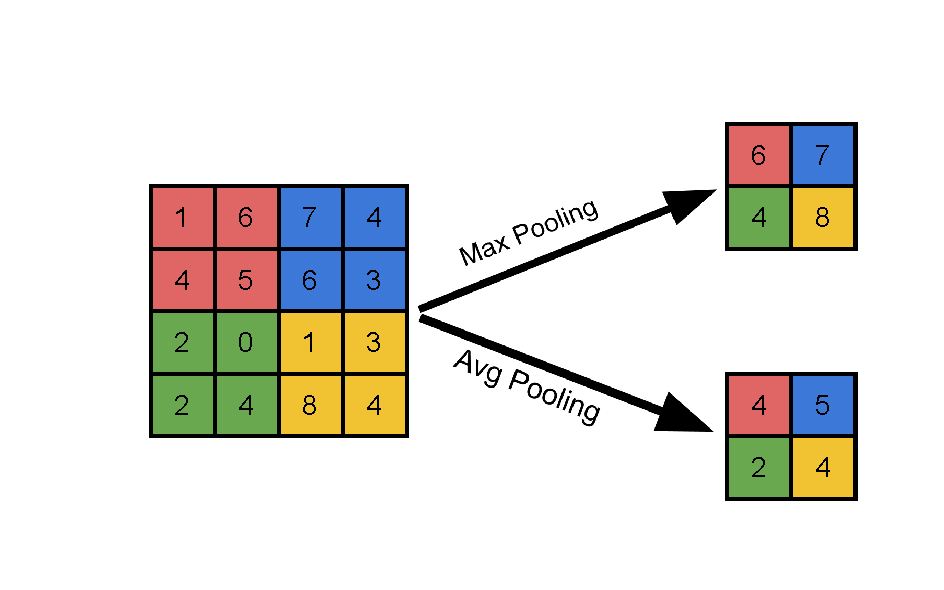
\includegraphics[clip, width=0.7\columnwidth]{figures/deeplearning/Pooling.pdf}
  \end{center}
  
  %\vspace*{-6pt}
  \caption[Pooling Layer]{A Pooling Layer with size $2 \times 2$ and a stride of 2. The output on the top represents max pooling the output on the bottom average pooling.}
  \label{fig:Pooling}
  %\vspace*{-12pt}
\end{figure}

Let us look at how pooling layers work. Like convolutional layers they are only connected to a small rectangular receptive field, but they typically do not connect to the full depth of the previous layer - they only subsample the individual "images". Pooling layers have no weights associated to them. Instead they use a pooling function to aggregate the inputs. Usually the \textit{max} or the \textit{mean} function is used. Figure \ref{fig:Pooling} shows an example of a pooling layer with $2 \times 2$ kernels with a stride of 2. On the top we have the output of a \textit{max pooling layer}, which means that out of four values from the input image only the maximum will be propagated to the next layer and on the bottom is the output of a \textit{average pooling layer} which averages over all its inputs. While earlier networks often used average pooling, nowadays often only max pooling is used. 

\begin{figure}[ht]
    
  \begin{center}
      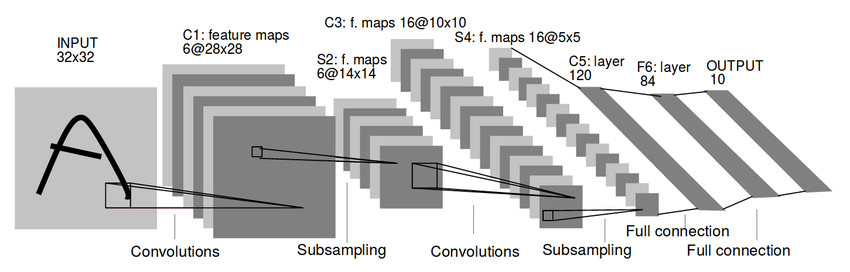
\includegraphics[clip, width=0.7\columnwidth]{figures/deeplearning/LeNetArch.png}
  \end{center}
  
  %\vspace*{-6pt}
  \caption[LeNet-5 Architecture]{The architecture of the first CNN LeNet-5 \cite{lecun1998gradient}. It was designed to recognise handwritten digits and used two convolutional and two pooling layers.}
  \label{fig:LeNet}
  %\vspace*{-12pt}
\end{figure}

Pooling layers typically use a stride which is equal to their own size. While pooling is very useful to save computational resources, pooling larger areas than $2 \times 2$ can lead to information loss, so pooling has to be used carefully. However in current CNN architectures, pooling layers are used after every convolutional layer. By using this structure the intermediate results get smaller and smaller and the repeated pooling results in a larger invariance against pixel shifts or even smaller rotations in the input image. 

Convolutioal networks usually end with one or more fully connected layers. We included a sketch of the original LeNet-5 architecture in Figure \ref{fig:LeNet} which demonstrates a typical CNN. Modern architectures are often larger in every aspect and often use convolutional layers in conjunction with residual connections to allow efficient training of very deep networks. Recent papers also suggest to only use convolutional layers (\textit{Fully Convolutional Networks} (FCNs)) for specific tasks like object detection \cite{long2015fully}. To further improve invariance against scaling and rotation, the feature output of multiple convolutional layers can be directly combined, which is called Feature Pyramid Network (FPN) \cite{lin2017feature}. 


% \section{Current Research} \label{sec:NNResearch}
% Since its rebirth around 2010, deep learning has been a field of extensive research with hundrets of papers published every years. Nowadays, deep learning techniques are incorporated into many end-user applications, especially when it comes to human interaction like speech recogition or search engines. Deep learning is also heavily used for modern automation tasks like self-driving cars. The large interest in improving these technologies has led to a situation, where records are broken every year and techniques quickly become outdated or at least develop into something more refined. In this Section we want to give some short insight    
